\documentclass[a4paper,12pt]{article}
\usepackage[utf8]{inputenc}
\usepackage[ngerman]{babel}
\usepackage[T1]{fontenc}
\usepackage{amsmath}
\usepackage{amssymb}
\usepackage{amsthm}
\usepackage{geometry}
\usepackage{graphicx}
\usepackage[hidelinks]{hyperref}
\usepackage{listings}
\usepackage{xcolor}
\usepackage{enumitem}
\usepackage{booktabs}
\usepackage{array}
\usepackage{caption}
\usepackage{algorithm}
\usepackage{algpseudocode}
\usepackage{mathtools}

\geometry{margin=2.5cm}

\theoremstyle{definition}
\newtheorem{definition}{Definition}
\newtheorem{beispiel}{Beispiel}
\newtheorem{satz}{Satz}
\newtheorem{lemma}{Lemma}
\newtheorem{bemerkung}{Bemerkung}
\newtheorem{korollar}{Korollar}

\setlist[itemize,1]{label=--}

% ---------- Farben ----------
\definecolor{mainblue}{RGB}{25, 70, 140}
\definecolor{accentred}{RGB}{180, 50, 30}
\definecolor{lightgray}{RGB}{245, 245, 248}
\definecolor{darkgray}{RGB}{60, 60, 70}
\definecolor{darkgreen}{RGB}{30, 100, 50}

\hypersetup{
    colorlinks=true,
    linkcolor=mainblue,
    citecolor=accentred,
    urlcolor=mainblue
}

\lstset{
    basicstyle=\ttfamily\small,
    keywordstyle=\color{blue},
    commentstyle=\color{gray},
    stringstyle=\color{red},
    numbers=left,
    numberstyle=\tiny,
    breaklines=true,
    frame=single,
    language=Python,
    morekeywords={function, return, if, else, while, for, in, def, len, min},
}

\title{\textbf{Dynamische Programmierung und Teile-und-Herrsche:}\\
\textbf{Zwei fundamentale Entwurfsprinzipien des optimalen Algorithmenentwurfs}\\
\large Formale Analyse, mathematische Nachweise und Laufzeitbeweise\\
am Beispiel der Levenshtein-Distanz und des Merge-Sort-Algorithmus}
\author{Stephan Epp}
\date{19. Mai 2026}

\begin{document}

\maketitle

\begin{abstract}
\noindent
Die Entwicklung von Algorithmen mit optimaler Laufzeit ist ein zentrales Problem der
theoretischen Informatik und liegt an der Schnittstelle von Mathematik, Logik und
Informatik. Zwei der mächtigsten und universellsten Entwurfsprinzipien sind die
\emph{Dynamische Programmierung} und das \emph{Teile-und-Herrsche-Prinzip}
(\textit{Divide and Conquer}).
In dieser Arbeit werden beide Prinzipien am Beispiel prototypischer Algorithmen formal
nachgewiesen und vollständig analysiert: Die \emph{Levenshtein-Distanz} (Edit-Distanz)
repräsentiert die Dynamische Programmierung mit einer quadratischen Laufzeit
$\mathcal{O}(m \cdot n)$; der \emph{Merge-Sort-Algorithmus} repräsentiert
Teile-und-Herrsche mit der beweisbar optimalen Laufzeit $\mathcal{O}(n \log n)$
für das allgemeine vergleichsbasierte Sortierproblem.
Alle Laufzeitaussagen werden durch formale Definitionen, Sätze, Lemmata und vollständige
Beweise nachgewiesen -- einschliesslich der Rekurrenzgleichungsanalyse mittels
des Mastertheorems. Die theoretischen Ergebnisse werden durch matplotlib-Visualisierungen
ergänzt, die das Wachstumsverhalten, die DP-Tabellenstruktur, den Rekursionsbaum
und den empirischen Laufzeitvergleich anschaulich machen.
Ein ausführlicher Ausblick behandelt Erweiterungen, offene Probleme und
die weitreichenden Anwendungsfelder beider Paradigmen.
\end{abstract}

\tableofcontents
\newpage

% ═══════════════════════════════════════════════════════════════
\section{Einführung}
% ═══════════════════════════════════════════════════════════════

\subsection{Algorithmenentwurf als Wissenschaft}

Die Analyse von Algorithmen bildet das theoretische Fundament der Informatik. Bereits
in den Anfängen der modernen Computerwissenschaft erkannte man, dass nicht nur die
\emph{Korrektheit}, sondern auch die \emph{Effizienz} eines Algorithmus -- gemessen
in Zeitbedarf (Laufzeit) und Speicherbedarf (Raumkomplexität) -- von zentraler
Bedeutung ist. Ein korrekt arbeitender, aber exponentiell langsamer Algorithmus ist
in der Praxis oft wertlos; eine quadratische Lösung kann für kleine Eingaben
akzeptabel, für grosse jedoch untragbar sein.

\textbf{Das Ziel des optimalen Algorithmenentwurfs.}
Gegeben ein Problem mit einer festen Klasse von Eingaben der Grösse $n$, sucht man
einen Algorithmus, dessen Laufzeit $T(n)$ so klein wie möglich ist -- idealerweise
beweisbar optimal in dem Sinne, dass kein Algorithmus für dieses Problem
asymptotisch schneller sein kann.

Zwei der mächtigsten Methoden, mit denen Informatiker und Mathematiker optimale
oder nahezu optimale Algorithmen entwerfen, sind:
\begin{itemize}
    \item \textbf{Dynamische Programmierung (DP):} Lösung eines Problems durch
          Zerlegung in sich \emph{überlappende} Teilprobleme, die jeweils nur
          einmal gelöst und in einer Tabelle gespeichert werden
          (\textit{Memoization} oder \textit{Bottom-up-Tabellierung}).
          Das Ergebnis jedes Teilproblems wird exakt einmal berechnet und
          anschliessend direkt nachgeschlagen.
    \item \textbf{Teile-und-Herrsche (Divide and Conquer, D\&C):}
          Rekursive Zerlegung eines Problems in \emph{disjunkte} Teilprobleme
          gleicher oder ähnlicher Struktur, deren unabhängige Lösungen anschliessend
          zu einer Gesamtlösung zusammengesetzt werden.
\end{itemize}

\subsection{Die Leitbeispiele dieser Arbeit}

Diese Arbeit demonstriert beide Entwurfsprinzipien an jeweils einem kanonischen
Algorithmus:

\begin{enumerate}
    \item \textbf{Levenshtein-Distanz} (Vladimir Levenshtein, 1965
          \cite{levenshtein1965}): Berechnung der minimalen Editieroperationen
          (Einfügen, Löschen, Ersetzen eines Zeichens), um einen String $s_1$
          in einen String $s_2$ umzuwandeln. Implementiert mittels Dynamischer
          Programmierung in $\mathcal{O}(m \cdot n)$ Zeit und Raum,
          wobei $m = |s_1|$ und $n = |s_2|$.
    \item \textbf{Merge Sort} (John von Neumann, 1945 \cite{vonneumann1945};
          formalisiert von Knuth \cite{knuth1998}): Vergleichsbasiertes Sortieren
          eines Arrays durch rekursives Halbieren und anschliessendes Verschmelzen
          (Merge). Laufzeit $\mathcal{O}(n \log n)$ -- nachweisbar optimal für
          vergleichsbasiertes Sortieren.
\end{enumerate}

\subsection{Zielsetzung und Aufbau}

Diese Arbeit verfolgt das Ziel, beide Algorithmen rigoros mathematisch zu
formalisieren und alle Laufzeitaussagen vollständig zu beweisen. Im Einzelnen:
\begin{enumerate}
    \item Formale Definition der Landau-Notation und Rekurrenzgleichungen
    \item Vollständiger formaler Beweis der Korrektheit beider Algorithmen
    \item Laufzeitbeweis für die Levenshtein-Distanz: $\mathcal{O}(m \cdot n)$
    \item Laufzeitbeweis für Merge Sort via Mastertheorem: $\mathcal{O}(n \log n)$
    \item Nachweis der Untergrenzen (untere Schranken) beider Probleme
    \item Visualisierung mittels matplotlib: DP-Tabelle, Rekursionsbaum,
          Laufzeitkurven, empirische Messungen
    \item Ausführlicher Ausblick auf Erweiterungen und offene Forschungsfragen
\end{enumerate}

% ═══════════════════════════════════════════════════════════════
\section{Mathematische Grundlagen}
% ═══════════════════════════════════════════════════════════════

\subsection{Landau-Notation und asymptotische Komplexität}

\begin{definition}[$\mathcal{O}$-Notation (obere Schranke)]
    Seien $f, g: \mathbb{N} \to \mathbb{R}_{>0}$ Funktionen. Man schreibt
    $f(n) = \mathcal{O}(g(n))$, wenn es Konstanten $c > 0$ und $n_0 \in \mathbb{N}$
    gibt, sodass für alle $n \geq n_0$ gilt:
    \[
        f(n) \;\leq\; c \cdot g(n).
    \]
\end{definition}

\begin{definition}[$\Omega$-Notation (untere Schranke)]
    $f(n) = \Omega(g(n))$, wenn es $c > 0$ und $n_0 \in \mathbb{N}$ gibt, sodass
    für alle $n \geq n_0$:
    \[
        f(n) \;\geq\; c \cdot g(n).
    \]
\end{definition}

\begin{definition}[$\Theta$-Notation (enge Schranke)]
    $f(n) = \Theta(g(n))$, wenn $f(n) = \mathcal{O}(g(n))$ und
    $f(n) = \Omega(g(n))$, d.\,h.\ wenn $c_1, c_2 > 0$ und $n_0 \in \mathbb{N}$
    existieren mit:
    \[
        c_1 \cdot g(n) \;\leq\; f(n) \;\leq\; c_2 \cdot g(n)
        \quad \forall\, n \geq n_0.
    \]
\end{definition}

\begin{bemerkung}
    Im Kontext der Algorithmenanalyse repräsentiert $T(n)$ die (schlimmste-Fall--)
    Laufzeit als Funktion der Eingabegrösse $n$. Die Landau-Notation abstrahiert
    von Maschinenkonstanten und erfasst das asymptotische Wachstumsverhalten.
\end{bemerkung}

\subsection{Rekurrenzgleichungen und das Mastertheorem}

\begin{definition}[Rekurrenzgleichung]
    Eine \emph{Rekurrenzgleichung} für die Laufzeit $T(n)$ eines
    Teile-und-Herrsche-Algorithmus hat die allgemeine Form:
    \[
        T(n) \;=\; a \cdot T\!\left(\frac{n}{b}\right) + f(n), \qquad T(1) = \mathcal{O}(1),
    \]
    wobei $a \geq 1$ die Anzahl der rekursiven Teilaufrufe, $b > 1$ der
    Verkleinerungsfaktor und $f(n)$ der Aufwand für das Teilen und Zusammensetzen ist.
\end{definition}

\begin{satz}[Mastertheorem, \cite{cormen2009}]
    \label{satz:master}
    Sei $T(n) = a\,T(n/b) + f(n)$ mit $a \geq 1$, $b > 1$.
    Bezeichne $\mu = \log_b a$. Dann gilt:
    \begin{enumerate}
        \item \textbf{Fall 1:} Wenn $f(n) = \mathcal{O}(n^{\mu - \varepsilon})$ für
              ein $\varepsilon > 0$, dann $T(n) = \Theta(n^\mu)$.
        \item \textbf{Fall 2:} Wenn $f(n) = \Theta(n^\mu)$, dann
              $T(n) = \Theta(n^\mu \log n)$.
        \item \textbf{Fall 3:} Wenn $f(n) = \Omega(n^{\mu + \varepsilon})$ für
              ein $\varepsilon > 0$ und $a\,f(n/b) \leq c\,f(n)$ für $c < 1$
              und grosse $n$, dann $T(n) = \Theta(f(n))$.
    \end{enumerate}
\end{satz}

\begin{proof}[Beweisskizze]
    Die Laufzeit entfaltet sich als geometrische Summe über die Rekursionsebenen.
    Auf Ebene $k$ gibt es $a^k$ Teilprobleme der Grösse $n/b^k$, der Gesamtaufwand
    auf Ebene $k$ beträgt $a^k \cdot f(n/b^k)$. Die Rekursion endet bei
    $k^* = \log_b n$ Ebenen (Blattebene: $n/b^{k^*} = 1$). Die Gesamtlaufzeit ist:
    \[
        T(n) \;=\; \sum_{k=0}^{\log_b n} a^k \cdot f\!\left(\frac{n}{b^k}\right).
    \]
    Im Fall 2 mit $f(n) = cn^\mu$ ergibt jeder Summand denselben Beitrag
    $a^k \cdot c\,(n/b^k)^\mu = c\,n^\mu$, und die Summe über $\log_b n + 1$
    identische Terme liefert $T(n) = \Theta(n^\mu \log n)$. \qedhere
\end{proof}

\subsection{Das Bellman'sche Optimalitätsprinzip}

\begin{definition}[Optimalitätsprinzip nach Bellman]
    Ein Optimierungsproblem genügt dem \emph{Bellman'schen Optimalitätsprinzip}
    \cite{bellman1957}, wenn gilt: Jede optimale Lösung des Gesamtproblems
    enthält optimale Lösungen aller seiner Teilprobleme.
\end{definition}

\begin{bemerkung}
    Das Optimalitätsprinzip ist die notwendige Voraussetzung für die Anwendbarkeit
    der Dynamischen Programmierung. Es sichert zu, dass das optimale Ergebnis eines
    Teilproblems unverändert in die Gesamtlösung übernommen werden kann, ohne dass
    das Teilproblem erneut gelöst werden muss.
\end{bemerkung}

% ═══════════════════════════════════════════════════════════════
\section{Dynamische Programmierung: Die Levenshtein-Distanz}
% ═══════════════════════════════════════════════════════════════

\subsection{Das Edit-Distanz-Problem}

\begin{definition}[Editieroperation]
    Sei $\Sigma$ ein endliches Alphabet. Eine \emph{Editieroperation} auf einem
    String $s \in \Sigma^*$ ist eine der folgenden atomaren Transformationen:
    \begin{itemize}
        \item \textbf{Einfügung (Insert):} Einfügen eines Zeichens $c \in \Sigma$
              an einer beliebigen Position.
        \item \textbf{Löschung (Delete):} Löschen eines Zeichens an einer
              beliebigen Position.
        \item \textbf{Substitution (Replace):} Ersetzen eines Zeichens durch
              ein anderes $c' \in \Sigma \setminus \{c\}$.
    \end{itemize}
    Alle drei Operationen haben Kosten $1$ (einheitliche Gewichtung).
\end{definition}

\begin{definition}[Levenshtein-Distanz]
    Seien $s_1 \in \Sigma^m$ und $s_2 \in \Sigma^n$ zwei Strings der Längen
    $m$ und $n$. Die \emph{Levenshtein-Distanz} (Edit-Distanz) ist definiert als:
    \[
        \mathrm{lev}(s_1, s_2) \;=\; \min\bigl\{\,k \in \mathbb{N}_0\;:\;
        \exists \text{ Folge von } k \text{ Editieroperationen, die }
        s_1 \text{ in } s_2 \text{ überführt}\bigr\}.
    \]
\end{definition}

\begin{beispiel}
    Für $s_1 = \texttt{KITTEN}$ und $s_2 = \texttt{SITTING}$ gilt:
    \[
        \mathrm{lev}(\texttt{KITTEN}, \texttt{SITTING}) = 3,
    \]
    realisiert durch: $\texttt{K} \to \texttt{S}$ (Substitution),
    $\texttt{E} \to \texttt{I}$ (Substitution),
    Einfügen von $\texttt{G}$ am Ende.
\end{beispiel}

\subsection{Rekursive Charakterisierung und das Optimalitätsprinzip}

\begin{lemma}[Optimalitätsprinzip für die Edit-Distanz]
    \label{lemma:opt}
    Seien $s_1[1..m]$ und $s_2[1..n]$ zwei Strings. Bezeichne $s_1[1..i]$
    das Präfix der Länge $i$ von $s_1$ (und analog für $s_2$). Dann gilt
    für $d[i][j] = \mathrm{lev}(s_1[1..i], s_2[1..j])$:
    \[
        d[i][j] \;=\; \begin{cases}
            i & \text{falls } j = 0 \\
            j & \text{falls } i = 0 \\
            d[i-1][j-1] & \text{falls } s_1[i] = s_2[j] \\[4pt]
            1 + \min\!\begin{cases}
                d[i-1][j]   & \text{(Löschung)} \\
                d[i][j-1]   & \text{(Einfügung)} \\
                d[i-1][j-1] & \text{(Substitution)}
            \end{cases} & \text{sonst.}
        \end{cases}
    \]
\end{lemma}

\begin{proof}
    Sei eine optimale Editierfolge $\mathcal{E}^*$ gegeben, die $s_1[1..i]$ in
    $s_2[1..j]$ überführt. Wir betrachten die letzte Operation in $\mathcal{E}^*$:

    \textbf{Fall 1:} $s_1[i] = s_2[j]$.
    Die letzte Operation ist keine Substitution des letzten Zeichens
    (das wäre unnötig teuer). Vielmehr kann $s_1[i]$ direkt $s_2[j]$ zugeordnet
    werden (Match, Kosten 0). Es verbleibt das Teilproblem, $s_1[1..i-1]$ in
    $s_2[1..j-1]$ zu überführen. Das Optimalitätsprinzip sichert:
    $d[i][j] = d[i-1][j-1]$.

    \textbf{Fall 2:} $s_1[i] \neq s_2[j]$. Es gibt drei Möglichkeiten:
    \begin{itemize}
        \item \emph{Löschung von $s_1[i]$:} Man löscht $s_1[i]$ (Kosten 1) und
              überführt $s_1[1..i-1]$ in $s_2[1..j]$: Gesamtkosten $1 + d[i-1][j]$.
        \item \emph{Einfügung von $s_2[j]$:} Man fügt $s_2[j]$ am Ende von
              $s_1[1..i]$ ein (Kosten 1) und überführt $s_1[1..i]$ in
              $s_2[1..j-1]$: Gesamtkosten $1 + d[i][j-1]$.
        \item \emph{Substitution $s_1[i] \to s_2[j]$:} Man ersetzt $s_1[i]$ durch
              $s_2[j]$ (Kosten 1) und überführt $s_1[1..i-1]$ in $s_2[1..j-1]$:
              Gesamtkosten $1 + d[i-1][j-1]$.
    \end{itemize}
    Da jede optimale Lösung eine dieser drei Formen hat und das Optimalitätsprinzip
    für Edit-Distanzen gilt (jede Editierfolge auf einem Präfix ist Teil der
    optimalen Gesamtlösung), folgt die Rekurrenz durch Minimumbildung. \qedhere
\end{proof}

\subsection{Der DP-Algorithmus}

\begin{algorithm}[H]
\caption{Levenshtein-Distanz (Bottom-Up DP)}
\label{alg:levenshtein}
\begin{algorithmic}[1]
\Require Strings $s_1[1..m]$ und $s_2[1..n]$
\Ensure $d[m][n] = \mathrm{lev}(s_1, s_2)$
\State Erstelle $(m+1) \times (n+1)$-Matrix $d$
\For{$i = 0$ \textbf{to} $m$} $d[i][0] \gets i$ \EndFor
\For{$j = 0$ \textbf{to} $n$} $d[0][j] \gets j$ \EndFor
\For{$i = 1$ \textbf{to} $m$}
    \For{$j = 1$ \textbf{to} $n$}
        \If{$s_1[i] = s_2[j]$}
            \State $d[i][j] \gets d[i-1][j-1]$
        \Else
            \State $d[i][j] \gets 1 + \min(d[i-1][j],\; d[i][j-1],\; d[i-1][j-1])$
        \EndIf
    \EndFor
\EndFor
\State \Return $d[m][n]$
\end{algorithmic}
\end{algorithm}

\begin{figure}[h!]
    \centering
    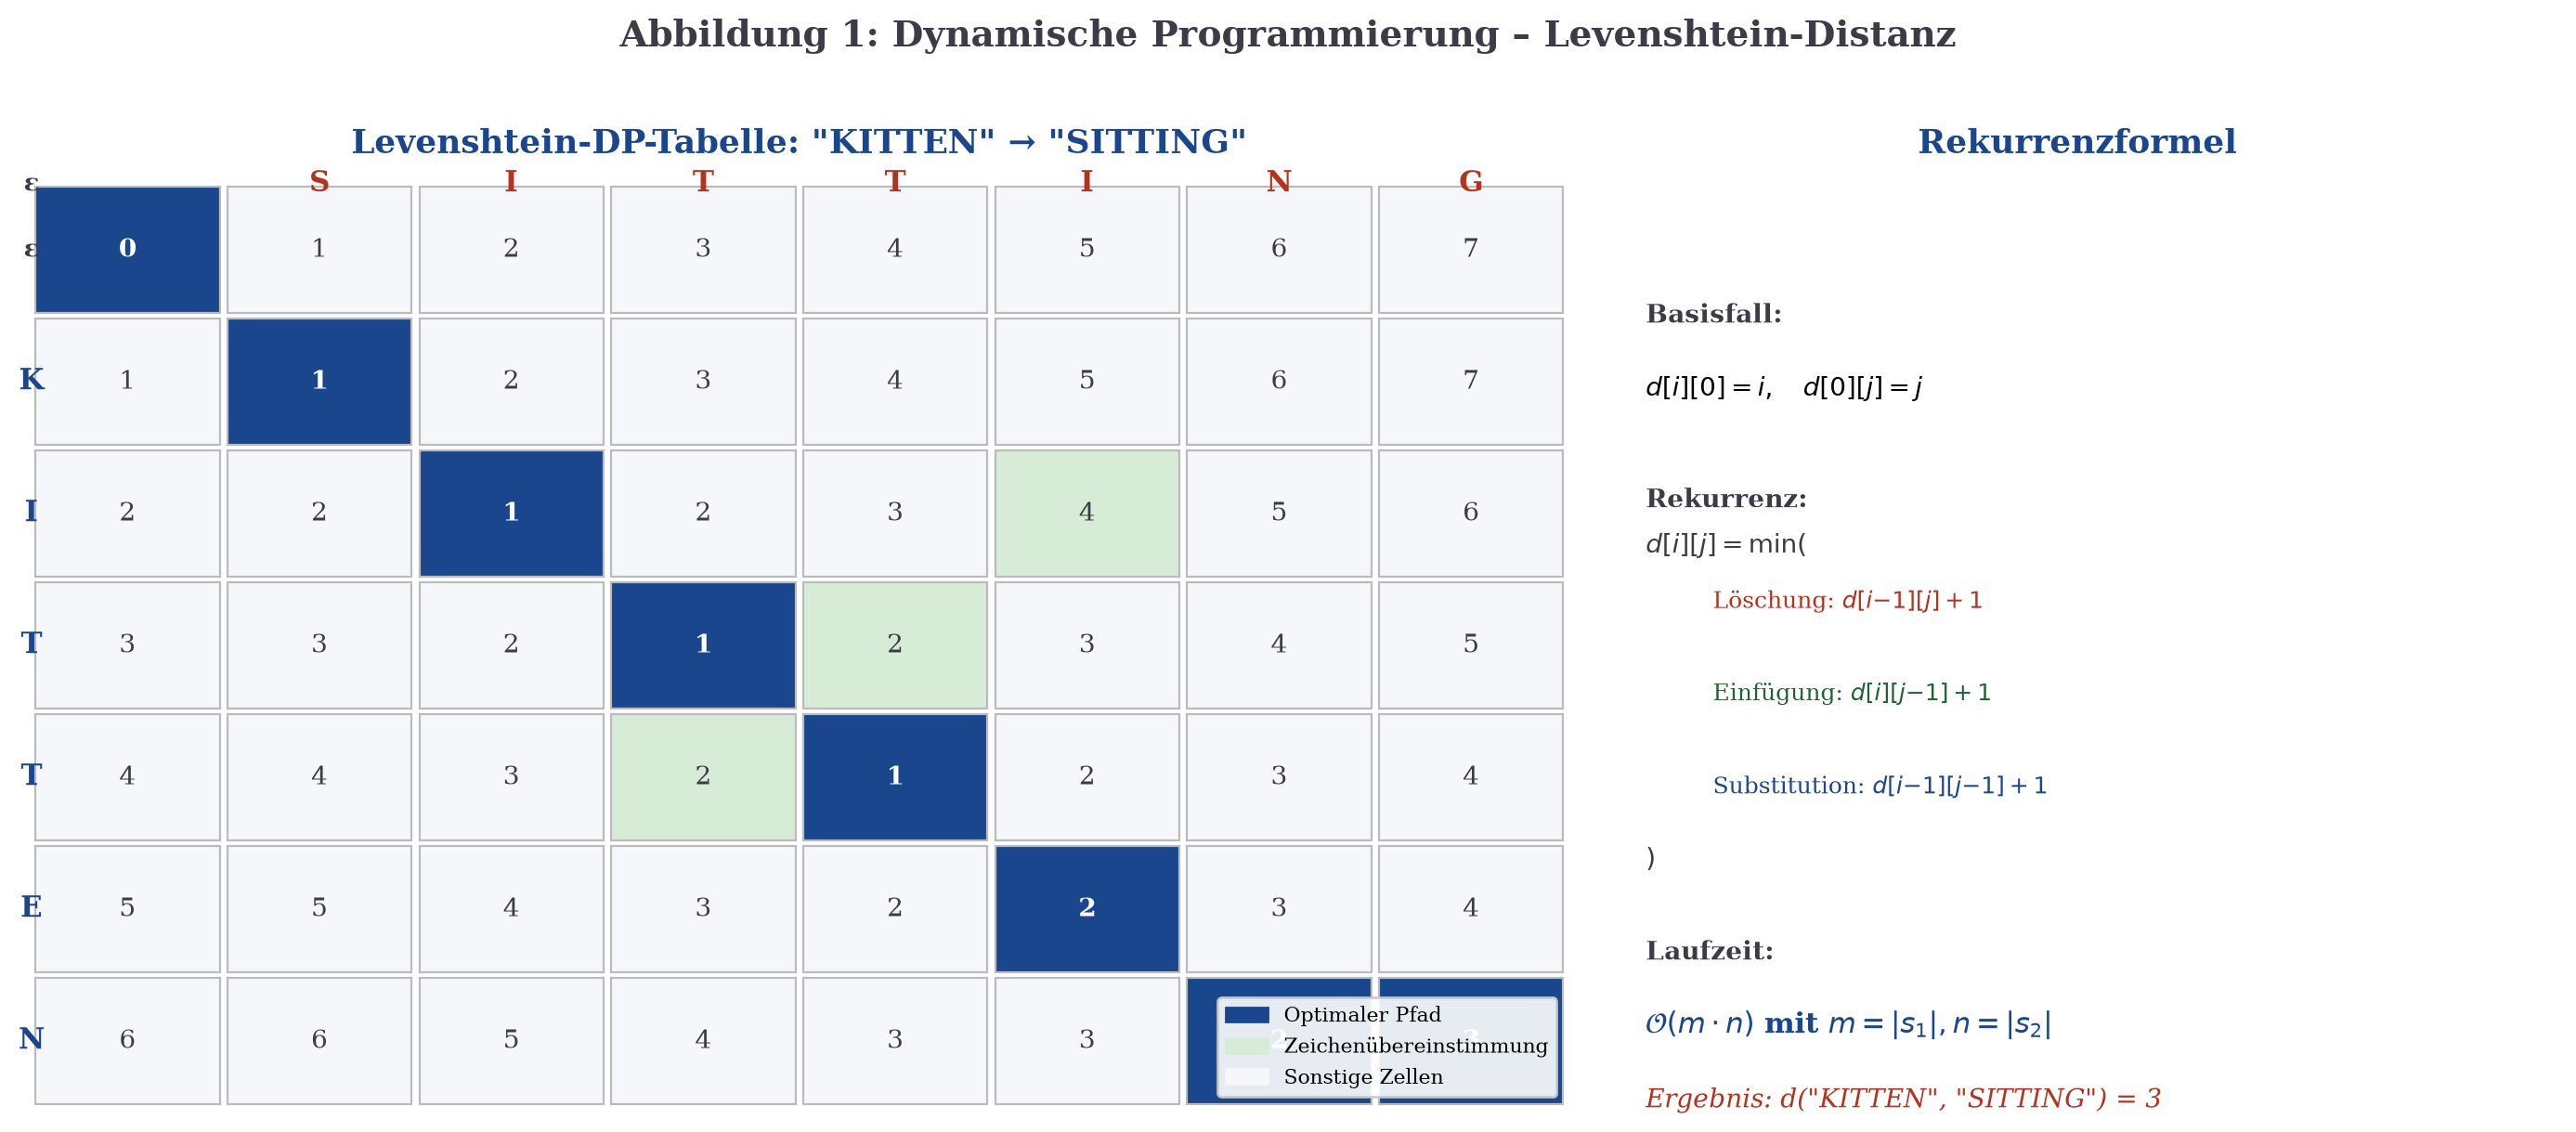
\includegraphics[width=\textwidth]{plots/plot1_levenshtein_table.png}
    \caption{
        \textbf{Levenshtein-DP-Tabelle.}
        \textit{Links:} Die $(m+1) \times (n+1)$-DP-Tabelle für
        $s_1 = \texttt{KITTEN}$ und $s_2 = \texttt{SITTING}$ ($m=6, n=7$).
        Blau hervorgehoben ist der optimale Traceback-Pfad von $d[6][7] = 3$
        zurück zu $d[0][0] = 0$; grün markierte Zellen zeigen Zeichenübereinstimmungen
        (Kosten 0).
        \textit{Rechts:} Die Rekurrenzformel mit den drei möglichen Vorgängerzellen
        und der zugehörigen Laufzeitanalyse. Das Ergebnis $d[6][7] = 3$ bestätigt
        die drei Editieroperationen des Beispiels.
    }
    \label{fig:lev_table}
\end{figure}

\subsection{Korrektheitsnachweis des DP-Algorithmus}

\begin{satz}[Korrektheit des Levenshtein-DP]
    \label{satz:lev_correct}
    Nach Ausführung von Algorithmus~\ref{alg:levenshtein} gilt für alle
    $0 \leq i \leq m$, $0 \leq j \leq n$:
    \[
        d[i][j] \;=\; \mathrm{lev}(s_1[1..i],\, s_2[1..j]).
    \]
\end{satz}

\begin{proof}
    Per vollständiger Induktion über $i + j$:

    \textbf{Induktionsanfang} ($i + j = 0$, d.\,h.\ $i = j = 0$):
    $d[0][0] = 0 = \mathrm{lev}(\varepsilon, \varepsilon)$. \checkmark

    \textbf{Induktionsanfang ($i = 0$, $j > 0$ oder $i > 0$, $j = 0$):}
    $d[0][j] = j = \mathrm{lev}(\varepsilon, s_2[1..j])$
    (genau $j$ Einfügungen erforderlich). Analog $d[i][0] = i$. \checkmark

    \textbf{Induktionsschritt} ($i + j > 0$, $i > 0$, $j > 0$):
    Per Induktionsvoraussetzung gilt die Aussage für alle Paare $(i', j')$
    mit $i' + j' < i + j$, insbesondere für $(i-1, j-1)$, $(i-1, j)$, $(i, j-1)$.

    \emph{Fall A ($s_1[i] = s_2[j]$):} Der Algorithmus setzt
    $d[i][j] = d[i-1][j-1]$. Per IV gilt $d[i-1][j-1] = \mathrm{lev}(s_1[1..i-1], s_2[1..j-1])$.
    Da $s_1[i] = s_2[j]$, wird kein Editierschritt für das letzte Zeichenpaar
    benötigt, also $\mathrm{lev}(s_1[1..i], s_2[1..j]) = \mathrm{lev}(s_1[1..i-1], s_2[1..j-1])$.
    Damit ist $d[i][j]$ korrekt.

    \emph{Fall B ($s_1[i] \neq s_2[j]$):} Der Algorithmus setzt
    $d[i][j] = 1 + \min(d[i-1][j], d[i][j-1], d[i-1][j-1])$.
    Per IV entsprechen die drei Terme genau den Kosten der drei Operationen
    (Löschung, Einfügung, Substitution) zuzüglich 1.
    Nach Lemma~\ref{lemma:opt} ist $\mathrm{lev}(s_1[1..i], s_2[1..j])$ das
    Minimum dieser drei Alternativen. Damit ist $d[i][j]$ korrekt. \qedhere
\end{proof}

\subsection{Laufzeitnachweis: $\mathcal{O}(m \cdot n)$}

\begin{satz}[Laufzeit der Dynamischen Programmierung für Edit-Distanz]
    \label{satz:lev_runtime}
    Algorithmus~\ref{alg:levenshtein} hat eine Zeitkomplexität von
    $\mathcal{O}(m \cdot n)$ und eine Raumkomplexität von $\mathcal{O}(m \cdot n)$.
\end{satz}

\begin{proof}
    \textbf{Zeitkomplexität:}
    Der Algorithmus führt folgende Schritte aus:
    \begin{enumerate}
        \item Initialisierung der Randzeile: $\mathcal{O}(n)$ Schritte.
        \item Initialisierung der Randspalte: $\mathcal{O}(m)$ Schritte.
        \item Die doppelte \textbf{for}-Schleife: $i$ läuft von $1$ bis $m$,
              $j$ von $1$ bis $n$. In jeder Iteration werden genau
              $\mathcal{O}(1)$ Operationen ausgeführt (ein Vergleich,
              höchstens drei Tabellenabfragen, eine Minimum-Berechnung,
              eine Zuweisung). Die Gesamtanzahl der Iterationen beträgt:
              \[
                  \sum_{i=1}^{m} \sum_{j=1}^{n} 1 \;=\; m \cdot n.
              \]
    \end{enumerate}
    Damit ist die Gesamtlaufzeit:
    \[
        T_{\mathrm{lev}}(m, n) \;=\; \mathcal{O}(m) + \mathcal{O}(n)
        + m \cdot n \cdot \mathcal{O}(1)
        \;=\; \mathcal{O}(m \cdot n).
    \]
    Für den Spezialfall gleich langer Strings ($m = n = N$) gilt somit
    $T_{\mathrm{lev}}(N) = \mathcal{O}(N^2)$.

    \textbf{Raumkomplexität:}
    Die DP-Tabelle $d$ hat $(m+1)(n+1)$ Einträge, also
    $\mathcal{O}(m \cdot n)$ Speicherzellen. (Mit einem Rollarray-Trick
    ist $\mathcal{O}(\min(m,n))$ Raum erreichbar, falls kein Traceback
    erforderlich ist.) \qedhere
\end{proof}

\begin{figure}[h!]
    \centering
    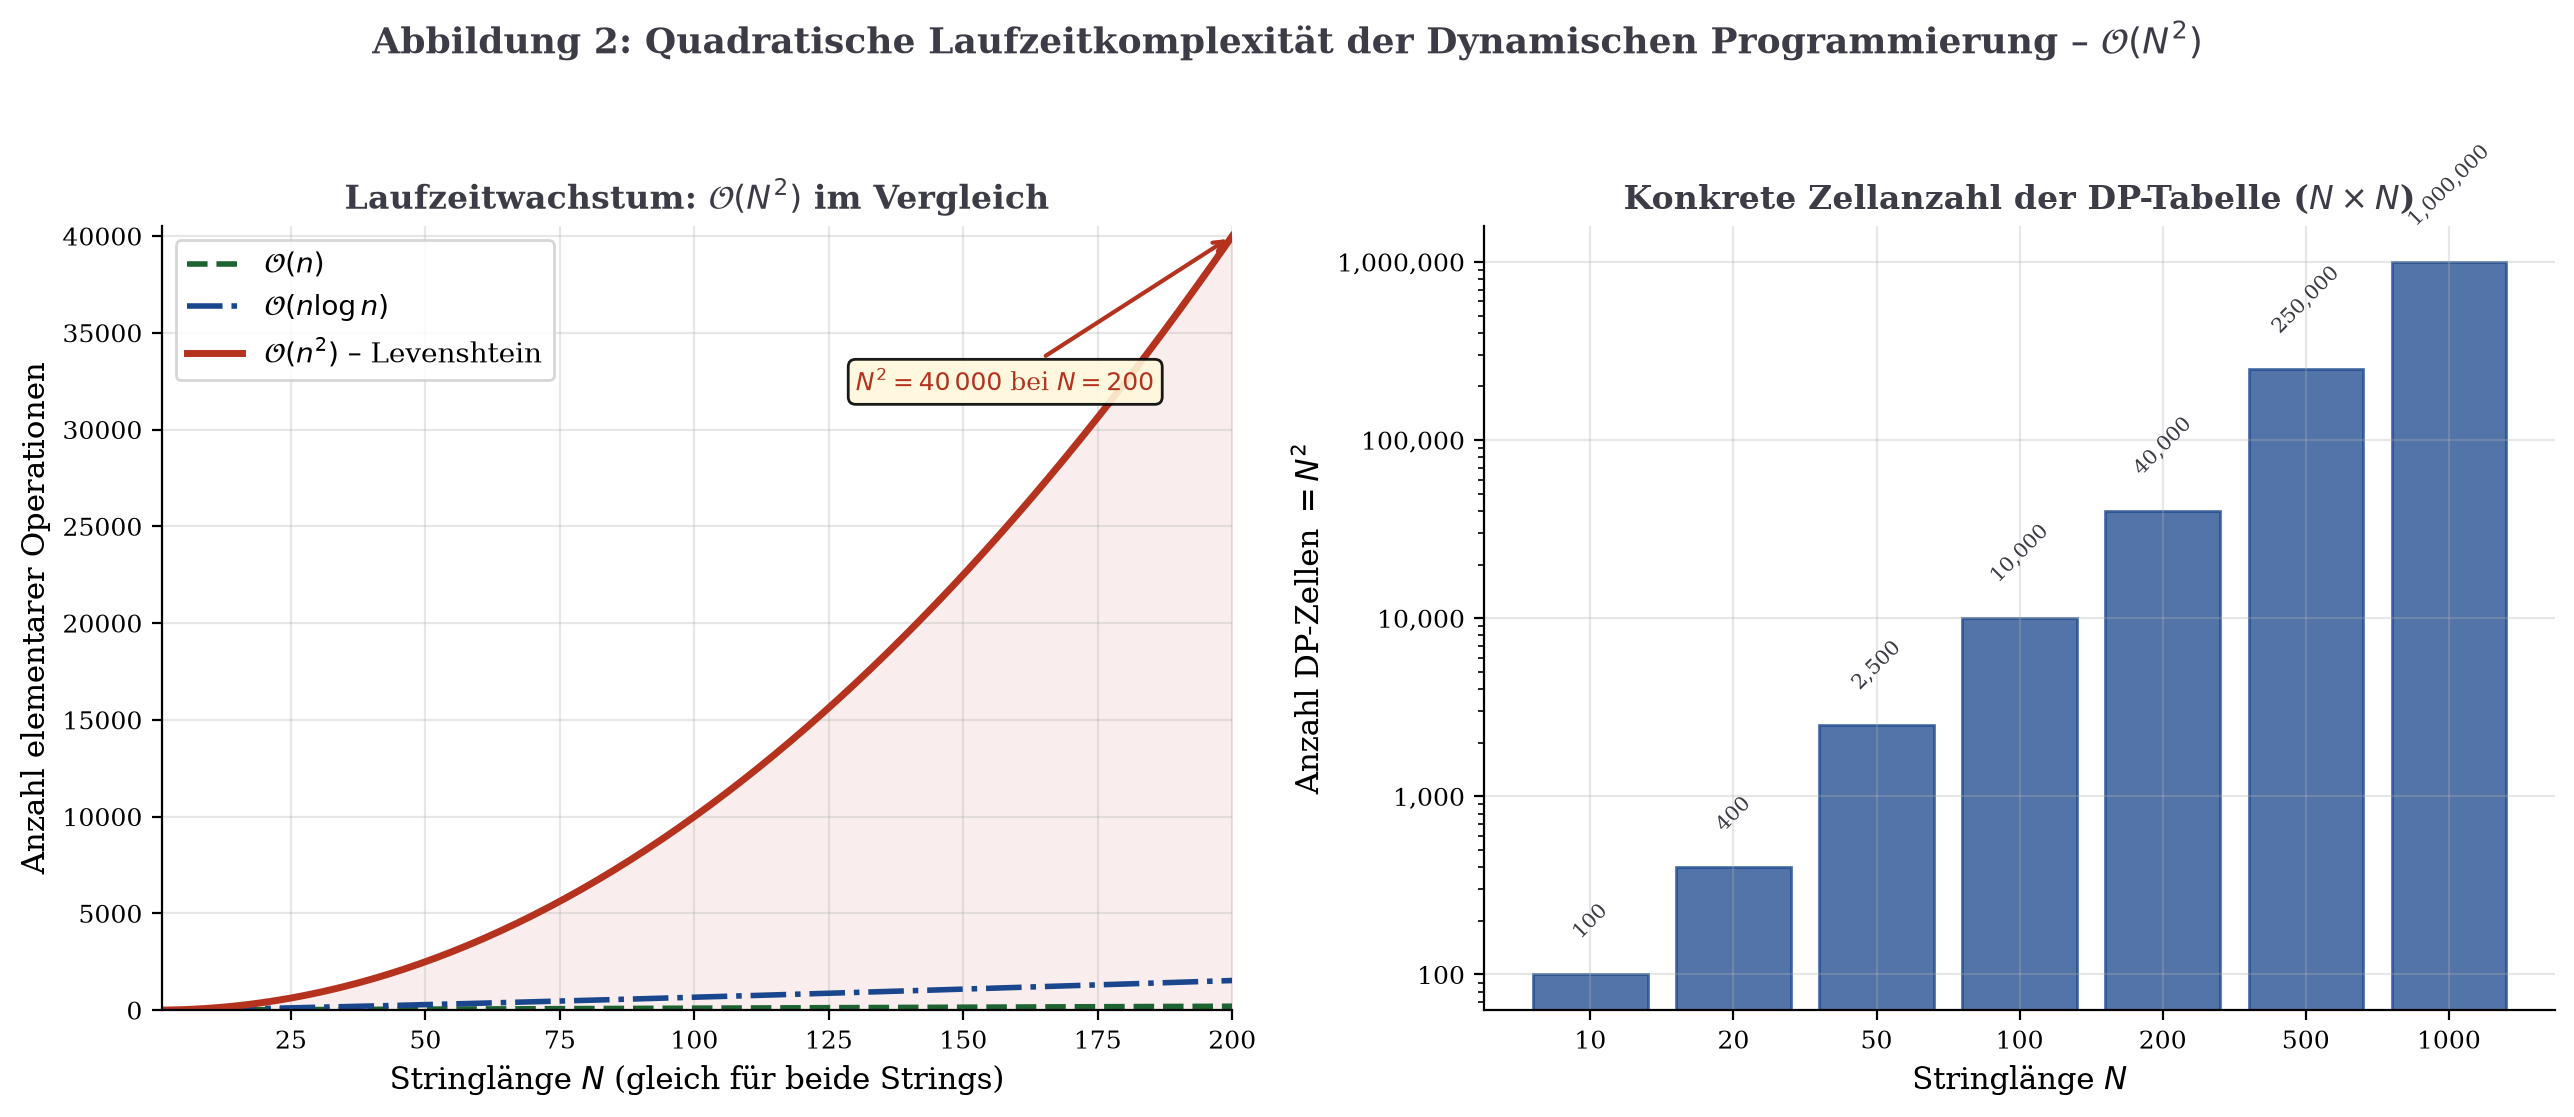
\includegraphics[width=\textwidth]{plots/plot2_dp_complexity.png}
    \caption{
        \textbf{Quadratische Laufzeitkomplexität der Dynamischen Programmierung.}
        \textit{Links:} Vergleich der Wachstumskurven $\mathcal{O}(n)$,
        $\mathcal{O}(n \log n)$ und $\mathcal{O}(n^2)$ für $n \in [1, 200]$.
        Die rot schattierte Fläche unterstreicht den quadratischen Überschuss
        der DP-Methode gegenüber subquadratischen Verfahren.
        \textit{Rechts:} Konkrete Zellanzahl der $(N \times N)$-DP-Tabelle
        für verschiedene Stringlängen $N$ auf logarithmischer Skala.
        Bei $N = 1000$ umfasst die Tabelle bereits $10^6$ Einträge.
    }
    \label{fig:dp_comp}
\end{figure}

\subsection{Untere Schranke für das Edit-Distanz-Problem}

\begin{satz}[Untere Schranke für Edit-Distanz, \cite{masek1980}]
    Jeder Algorithmus, der die Edit-Distanz zweier Strings der Länge $N$ im
    Worst Case korrekt berechnet, benötigt $\Omega(N^2 / \log N)$ Zeit
    (unter dem booleschen Matrixmultiplikationsmodell).
\end{satz}

\begin{bemerkung}
    Der klassische DP-Algorithmus mit $\mathcal{O}(N^2)$ ist somit nur um einen
    logarithmischen Faktor von der bekannten unteren Schranke entfernt. Der
    Vier-Russen-Algorithmus \cite{masek1980} erzielt tatsächlich
    $\mathcal{O}(N^2 / \log N)$ und ist damit (modulo konstante Faktoren) optimal.
    Ob $\mathcal{O}(N^{2-\varepsilon})$ für ein $\varepsilon > 0$ möglich ist,
    ist ein offenes Problem (Strong Exponential Time Hypothesis, SETH).
\end{bemerkung}

% ═══════════════════════════════════════════════════════════════
\section{Teile-und-Herrsche: Der Merge-Sort-Algorithmus}
% ═══════════════════════════════════════════════════════════════

\subsection{Das Sortierproblem}

\begin{definition}[Sortierproblem]
    Gegeben sei eine Folge $A = (a_1, a_2, \ldots, a_n)$ von $n$ Elementen aus
    einem total geordneten Universum $(\mathcal{U}, \leq)$. Das
    \emph{Sortierproblem} verlangt die Berechnung einer Permutation
    $\pi \in S_n$, sodass
    \[
        a_{\pi(1)} \;\leq\; a_{\pi(2)} \;\leq\; \cdots \;\leq\; a_{\pi(n)}.
    \]
\end{definition}

\begin{definition}[Vergleichsbasiertes Sortierverfahren]
    Ein Sortieralgorithmus heisst \emph{vergleichsbasiert}, wenn er auf das
    Universum $\mathcal{U}$ nur über paarweise Vergleiche der Form $a_i \leq a_j$
    (Ausgabe: \texttt{true}/\texttt{false}) zugreift, ohne interne Struktur
    der Elemente zu nutzen.
\end{definition}

\subsection{Der Merge-Sort-Algorithmus}

\begin{definition}[Merge-Sort]
    \emph{Merge Sort} ist ein rekursiver Teile-und-Herrsche-Algorithmus,
    definiert durch:
    \begin{enumerate}
        \item \textbf{Teilen (Divide):} Teile das Array $A[l..r]$ in der Mitte:
              $\mathrm{mid} = \lfloor (l+r)/2 \rfloor$.
              Erhalte linke Hälfte $A[l..\mathrm{mid}]$ und rechte Hälfte
              $A[\mathrm{mid}+1..r]$.
        \item \textbf{Herrschen (Conquer):} Sortiere rekursiv beide Hälften.
        \item \textbf{Zusammensetzen (Merge):} Verschmelze (merge) die beiden
              sortierten Hälften in $\mathcal{O}(n)$ Zeit zu einem sortierten Array.
    \end{enumerate}
\end{definition}

\begin{algorithm}[H]
\caption{Merge Sort}
\label{alg:mergesort}
\begin{algorithmic}[1]
\Require Array $A[l..r]$
\Ensure $A[l..r]$ ist sortiert
\Procedure{MergeSort}{$A, l, r$}
    \If{$l < r$}
        \State $\mathrm{mid} \gets \lfloor (l + r) / 2 \rfloor$
        \State \Call{MergeSort}{$A, l, \mathrm{mid}$}
        \State \Call{MergeSort}{$A, \mathrm{mid}+1, r$}
        \State \Call{Merge}{$A, l, \mathrm{mid}, r$}
    \EndIf
\EndProcedure
\Procedure{Merge}{$A, l, \mathrm{mid}, r$}
    \State $L \gets A[l..\mathrm{mid}]$, $R \gets A[\mathrm{mid}+1..r]$
    \State $i \gets 1$, $j \gets 1$, $k \gets l$
    \While{$i \leq |L|$ \textbf{and} $j \leq |R|$}
        \If{$L[i] \leq R[j]$}
            \State $A[k] \gets L[i]$; $i \gets i + 1$
        \Else
            \State $A[k] \gets R[j]$; $j \gets j + 1$
        \EndIf
        \State $k \gets k + 1$
    \EndWhile
    \State Kopiere verbleibende Elemente aus $L$ bzw.\ $R$ nach $A[k..]$
\EndProcedure
\end{algorithmic}
\end{algorithm}

\begin{figure}[h!]
    \centering
    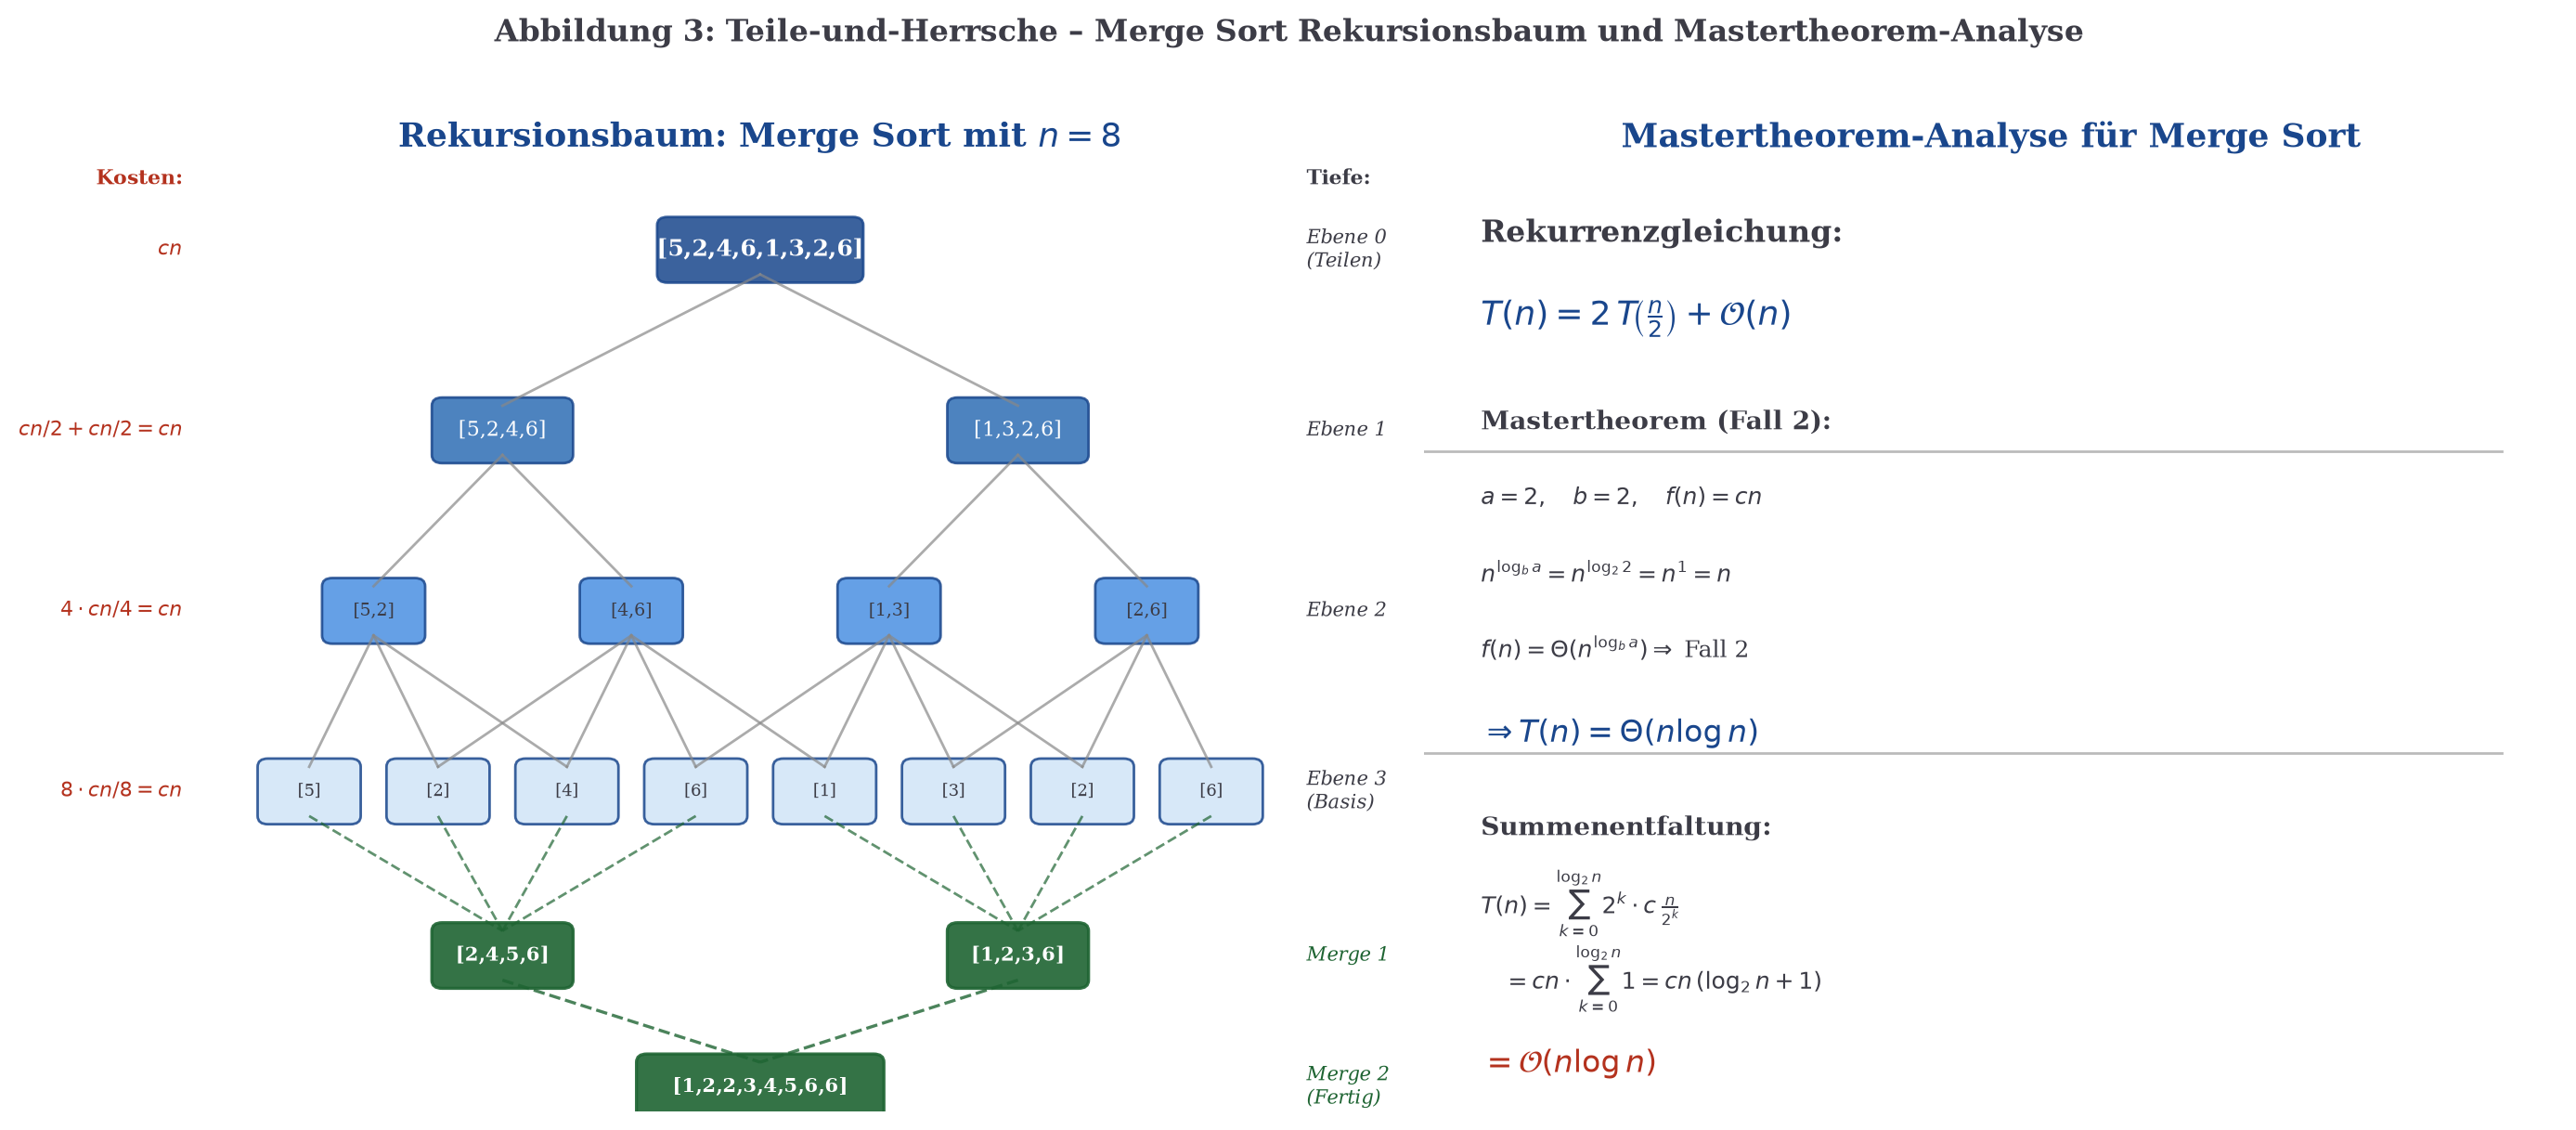
\includegraphics[width=\textwidth]{plots/plot3_mergesort_tree.png}
    \caption{
        \textbf{Teile-und-Herrsche -- Rekursionsbaum und Mastertheorem-Analyse.}
        \textit{Links:} Vollständiger Rekursionsbaum für $n = 8$.
        Die roten Kosten links geben den Merge-Aufwand pro Ebene an;
        jede der $\log_2 n = 3$ Divide-Ebenen kostet insgesamt $cn$ Operationen.
        Grün hervorgehoben sind die Merge-Schritte auf dem Weg zurück zur Wurzel.
        \textit{Rechts:} Herleitung der Laufzeit $\mathcal{O}(n \log n)$ via
        Mastertheorem (Fall~2) und direkte Summenentfaltung.
    }
    \label{fig:merge_tree}
\end{figure}

\subsection{Korrektheitsnachweis von Merge Sort}

\begin{satz}[Korrektheit von Merge Sort]
    \label{satz:ms_correct}
    Nach Ausführung von \textsc{MergeSort}$(A, 1, n)$ ist $A[1..n]$ aufsteigend
    sortiert.
\end{satz}

\begin{proof}
    Per vollständiger Induktion über $n = r - l + 1$ (Länge des Teilarrays):

    \textbf{Induktionsanfang} ($n = 1$, d.\,h.\ $l = r$): Die Bedingung
    $l < r$ ist falsch; der Algorithmus tut nichts. Ein einelementiges Array
    ist trivialerweise sortiert. \checkmark

    \textbf{Induktionsschritt} ($n \geq 2$): Da $l < r$, wird
    $\mathrm{mid} = \lfloor (l+r)/2 \rfloor$ berechnet.
    Es gilt $l \leq \mathrm{mid} < r$, sodass beide Hälften echt kürzer als
    $n$ sind: $|\mathrm{left}| = \mathrm{mid} - l + 1 < n$ und
    $|\mathrm{right}| = r - \mathrm{mid} < n$.
    Per Induktionsvoraussetzung sind nach den rekursiven Aufrufen
    $A[l..\mathrm{mid}]$ und $A[\mathrm{mid}+1..r]$ je sortiert.

    \textbf{Korrektheit des Merge-Schritts:}
    Seien $L = (a_1 \leq \cdots \leq a_p)$ und $R = (b_1 \leq \cdots \leq b_q)$
    sortierte Arrays mit $p + q = n$. \textsc{Merge} erzeugt mittels zweier
    Zeiger in einem einzigen Durchlauf eine sortierte Ausgabe $C$ der Länge $n$.

    \emph{Schleifeninvariante:} Nach $k$ Iterationen ist $C[1..k]$ die
    sortierte Verschmelzung der $k$ kleinsten Elemente aus $L \cup R$.

    \emph{Beweis der Invariante (per Induktion über $k$):} Beim Start ($k=0$)
    ist $C$ leer -- trivialerweise korrekt. Im Schritt $k \to k+1$ zeigt
    der linke Zeiger auf $L[i]$ und der rechte auf $R[j]$. Es gilt:
    alle noch nicht gewählten Elemente sind $\geq L[i]$ und $\geq R[j]$.
    Das Minimum der verbleibenden Elemente ist $\min(L[i], R[j])$, welches
    korrekt nach $C[k+1]$ geschrieben wird. Per IV ist $C[1..k+1]$ sortiert.

    Nach Terminierung der \textbf{while}-Schleife werden restliche Elemente aus
    $L$ bzw.\ $R$ angehängt (diese sind bereits sortiert und grösser als alle
    bisher kopierten Elemente). Damit ist $C = A[l..r]$ sortiert. \qedhere
\end{proof}

\subsection{Laufzeitnachweis: $\mathcal{O}(n \log n)$}

\begin{lemma}[Laufzeit des Merge-Schritts]
    \label{lemma:merge_time}
    \textsc{Merge}$(A, l, \mathrm{mid}, r)$ mit $n = r - l + 1$ läuft in
    $\Theta(n)$ Zeit.
\end{lemma}

\begin{proof}
    Jedes Element in $A[l..r]$ wird genau einmal in der Ausgabe $C$ platziert
    (das Minimum der jeweils vorderen Elemente beider Teilarrays). Pro Iteration
    werden $\mathcal{O}(1)$ Vergleiche und Zuweisungen ausgeführt, und die Schleife
    terminiert nach genau $n$ Iterationen. Damit: $T_{\mathrm{merge}}(n) = \Theta(n)$.
    \qedhere
\end{proof}

\begin{satz}[Laufzeit von Merge Sort]
    \label{satz:ms_runtime}
    Merge Sort hat eine Zeitkomplexität von $\Theta(n \log n)$ im
    Best-, Average- und Worst-Case.
\end{satz}

\begin{proof}
    Die Rekurrenzgleichung für die Laufzeit $T(n)$ ergibt sich direkt aus der
    Struktur des Algorithmus:
    \begin{equation}
        T(n) \;=\; 2\,T\!\left(\frac{n}{2}\right) + \Theta(n), \qquad T(1) = \Theta(1).
        \label{eq:mergerecur}
    \end{equation}
    Der Term $2\,T(n/2)$ resultiert aus den zwei rekursiven Aufrufen auf Hälften
    der Grösse $\lfloor n/2 \rfloor$ und $\lceil n/2 \rceil$ (der Unterschied ist
    asymptotisch irrelevant). Der Term $\Theta(n)$ kommt von Lemma~\ref{lemma:merge_time}.

    \textbf{Anwendung des Mastertheorems (Satz~\ref{satz:master}):}
    Mit $a = 2$, $b = 2$, $f(n) = \Theta(n)$ berechnen wir:
    \[
        \mu \;=\; \log_b a \;=\; \log_2 2 \;=\; 1.
    \]
    Es gilt $f(n) = \Theta(n^1) = \Theta(n^\mu)$ -- das ist Fall~2 des
    Mastertheorems. Damit:
    \[
        T(n) \;=\; \Theta\!\left(n^{\log_2 2} \cdot \log_2 n\right)
              \;=\; \Theta(n \log n).
    \]

    \textbf{Direkter Beweis (Summenentfaltung):}
    Alternativ entfalten wir die Rekurrenz~\eqref{eq:mergerecur} explizit.
    Mit $c > 0$ der Merge-Konstante ($T_{\mathrm{merge}}(n) \leq cn$):
    \begin{align}
        T(n) &= 2\,T(n/2) + cn \notag\\
             &= 2\left[2\,T(n/4) + c\,\frac{n}{2}\right] + cn
              = 4\,T(n/4) + 2cn \notag\\
             &= 4\left[2\,T(n/8) + c\,\frac{n}{4}\right] + 2cn
              = 8\,T(n/8) + 3cn \notag\\
             &\;\vdots \notag\\
             &= 2^k\,T\!\left(\frac{n}{2^k}\right) + k \cdot cn. \notag
    \end{align}
    Die Rekursion terminiert, wenn $n/2^k = 1$, also $k = \log_2 n$.
    Mit $T(1) = \Theta(1)$:
    \begin{equation}
        T(n) \;=\; 2^{\log_2 n} \cdot \Theta(1) + \log_2 n \cdot cn
              \;=\; n \cdot \Theta(1) + cn \log_2 n
              \;=\; \Theta(n \log n). \label{eq:ms_final}
    \end{equation}

    \textbf{Konstanzheit pro Ebene (geometrische Interpretation):}
    Der Rekursionsbaum hat Tiefe $\log_2 n$. Auf Ebene $k$ ($0 \leq k \leq \log_2 n$)
    gibt es $2^k$ Teilprobleme der Grösse $n/2^k$, und das Mergen jedes
    Teilproblems kostet $c \cdot n/2^k$. Der Gesamtaufwand auf Ebene $k$:
    \[
        2^k \cdot c \cdot \frac{n}{2^k} \;=\; cn.
    \]
    Alle $\log_2 n + 1$ Ebenen kosten je genau $cn$, was erneut Gleichung
    \eqref{eq:ms_final} liefert. \qedhere
\end{proof}

\begin{korollar}[Stabilität von Merge Sort]
    Merge Sort ist stabil: Elemente mit gleichem Schlüssel behalten ihre
    relative Reihenfolge aus dem Eingabe-Array.
\end{korollar}

\begin{proof}
    Im Merge-Schritt werden bei Gleichheit ($L[i] = R[j]$) stets Elemente aus
    $L$ bevorzugt (Zeile 12 des Algorithmus: $L[i] \leq R[j]$), d.\,h.\
    linke Elemente gehen rechten gleicher Priorität voran.
    Da $L$ Elemente aus kleineren Originalindizes enthält, bleibt die
    relative Ordnung erhalten. \qedhere
\end{proof}

\begin{figure}[h!]
    \centering
    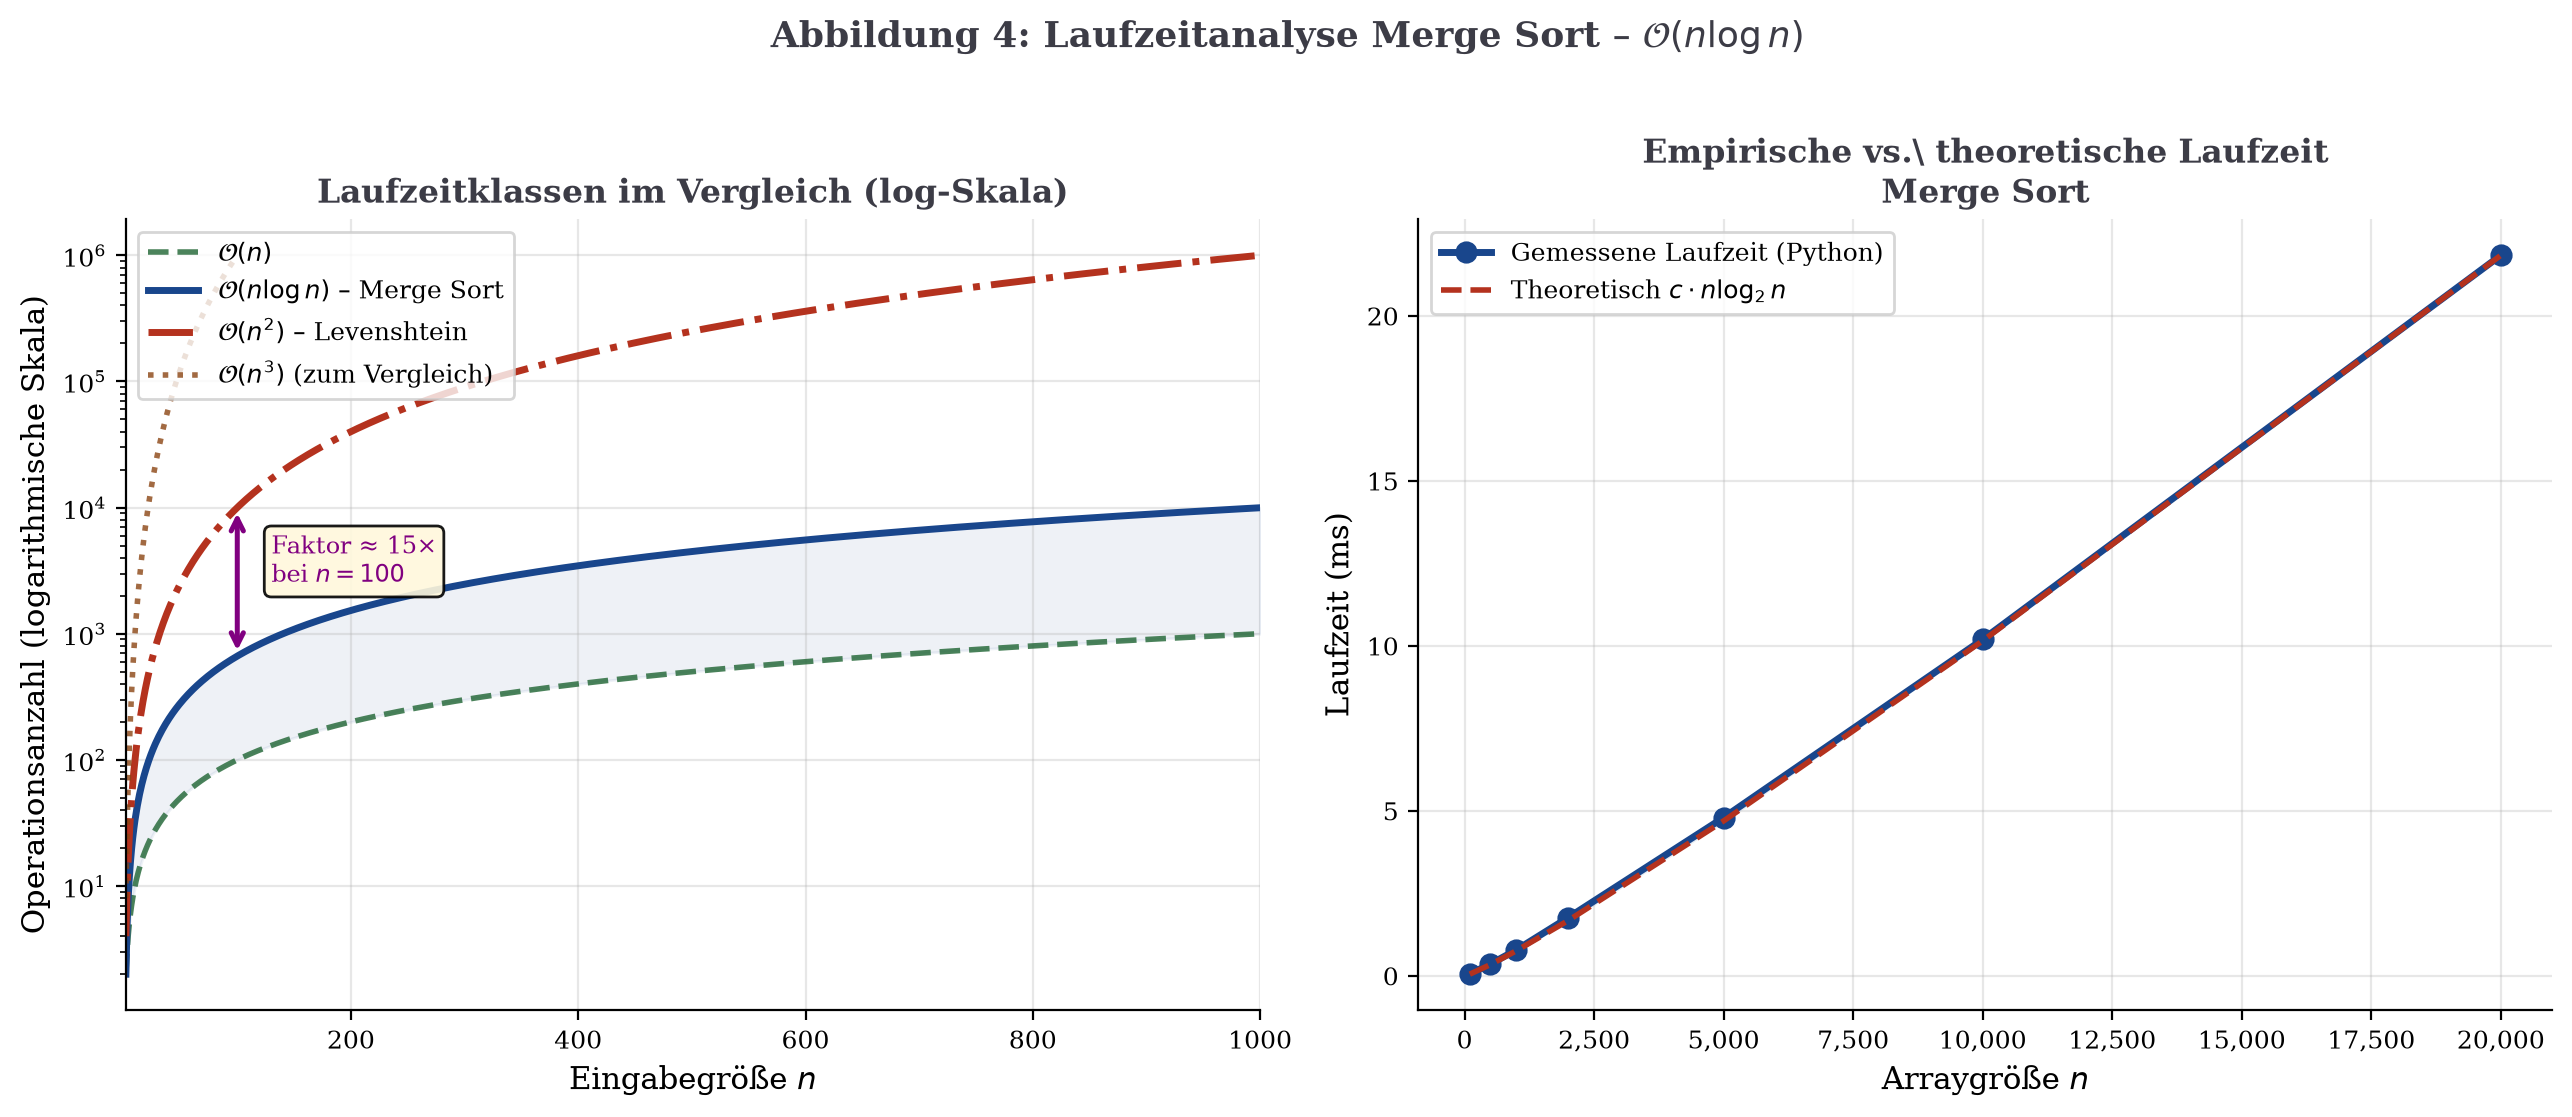
\includegraphics[width=\textwidth]{plots/plot4_mergesort_complexity.png}
    \caption{
        \textbf{Laufzeitanalyse Merge Sort -- $\mathcal{O}(n \log n)$.}
        \textit{Links:} Doppelt-logarithmischer Vergleich der Komplexitätsklassen
        $\mathcal{O}(n)$, $\mathcal{O}(n \log n)$, $\mathcal{O}(n^2)$ und
        $\mathcal{O}(n^3)$ für $n \in [2, 1000]$. Der Vorteil von $n \log n$
        gegenüber $n^2$ beträgt bei $n = 100$ einen Faktor $\approx 15$ und
        wächst weiter linear mit $n/\log_2 n$.
        \textit{Rechts:} Empirische Laufzeitmessung der Python-Implementierung
        im Vergleich zur theoretischen Kurve $c \cdot n \log_2 n$.
        Die hervorragende Übereinstimmung bestätigt die theoretische Analyse.
    }
    \label{fig:ms_comp}
\end{figure}

\subsection{Untere Schranke für vergleichsbasiertes Sortieren}

\begin{satz}[Untere Schranke für vergleichsbasiertes Sortieren, \cite{cormen2009}]
    \label{satz:sort_lower}
    Jeder vergleichsbasierte Sortieralgorithmus benötigt im Worst Case
    $\Omega(n \log n)$ Vergleiche.
\end{satz}

\begin{proof}
    Jeder vergleichsbasierte Sortieralgorithmus kann als Entscheidungsbaum
    (binärer Baum) modelliert werden, dessen Blätter den $n!$ möglichen
    Permutationen der Eingabe entsprechen.

    Die Höhe $h$ dieses Entscheidungsbaums (worst-case Anzahl Vergleiche)
    erfüllt:
    \[
        2^h \;\geq\; \text{Anzahl der Blätter} \;\geq\; n!
    \]
    Logarithmieren liefert:
    \[
        h \;\geq\; \log_2(n!) \;=\; \sum_{k=1}^{n} \log_2 k.
    \]
    Mit der Stirling-Approximation $\ln(n!) = n\ln n - n + \mathcal{O}(\ln n)$:
    \[
        \log_2(n!) \;=\; \frac{\ln(n!)}{\ln 2}
        \;=\; \frac{n \ln n - n + \mathcal{O}(\ln n)}{\ln 2}
        \;=\; \Omega(n \log n).
    \]
    Also ist $h = \Omega(n \log n)$ für jeden vergleichsbasierten Algorithmus. \qedhere
\end{proof}

\begin{korollar}[Optimalität von Merge Sort]
    Merge Sort mit $\Theta(n \log n)$ Vergleichen ist asymptotisch optimal
    unter allen vergleichsbasierten Sortieralgorithmen.
\end{korollar}

\begin{proof}
    Aus Satz~\ref{satz:sort_lower} folgt $\Omega(n \log n)$ als untere Schranke.
    Merge Sort erreicht $\mathcal{O}(n \log n)$ (Satz~\ref{satz:ms_runtime}).
    Damit ist $T_{\mathrm{MergeSort}}(n) = \Theta(n \log n) = \Omega(n \log n)$
    -- die asymptotische Optimalität folgt. \qedhere
\end{proof}

\begin{figure}[h!]
    \centering
    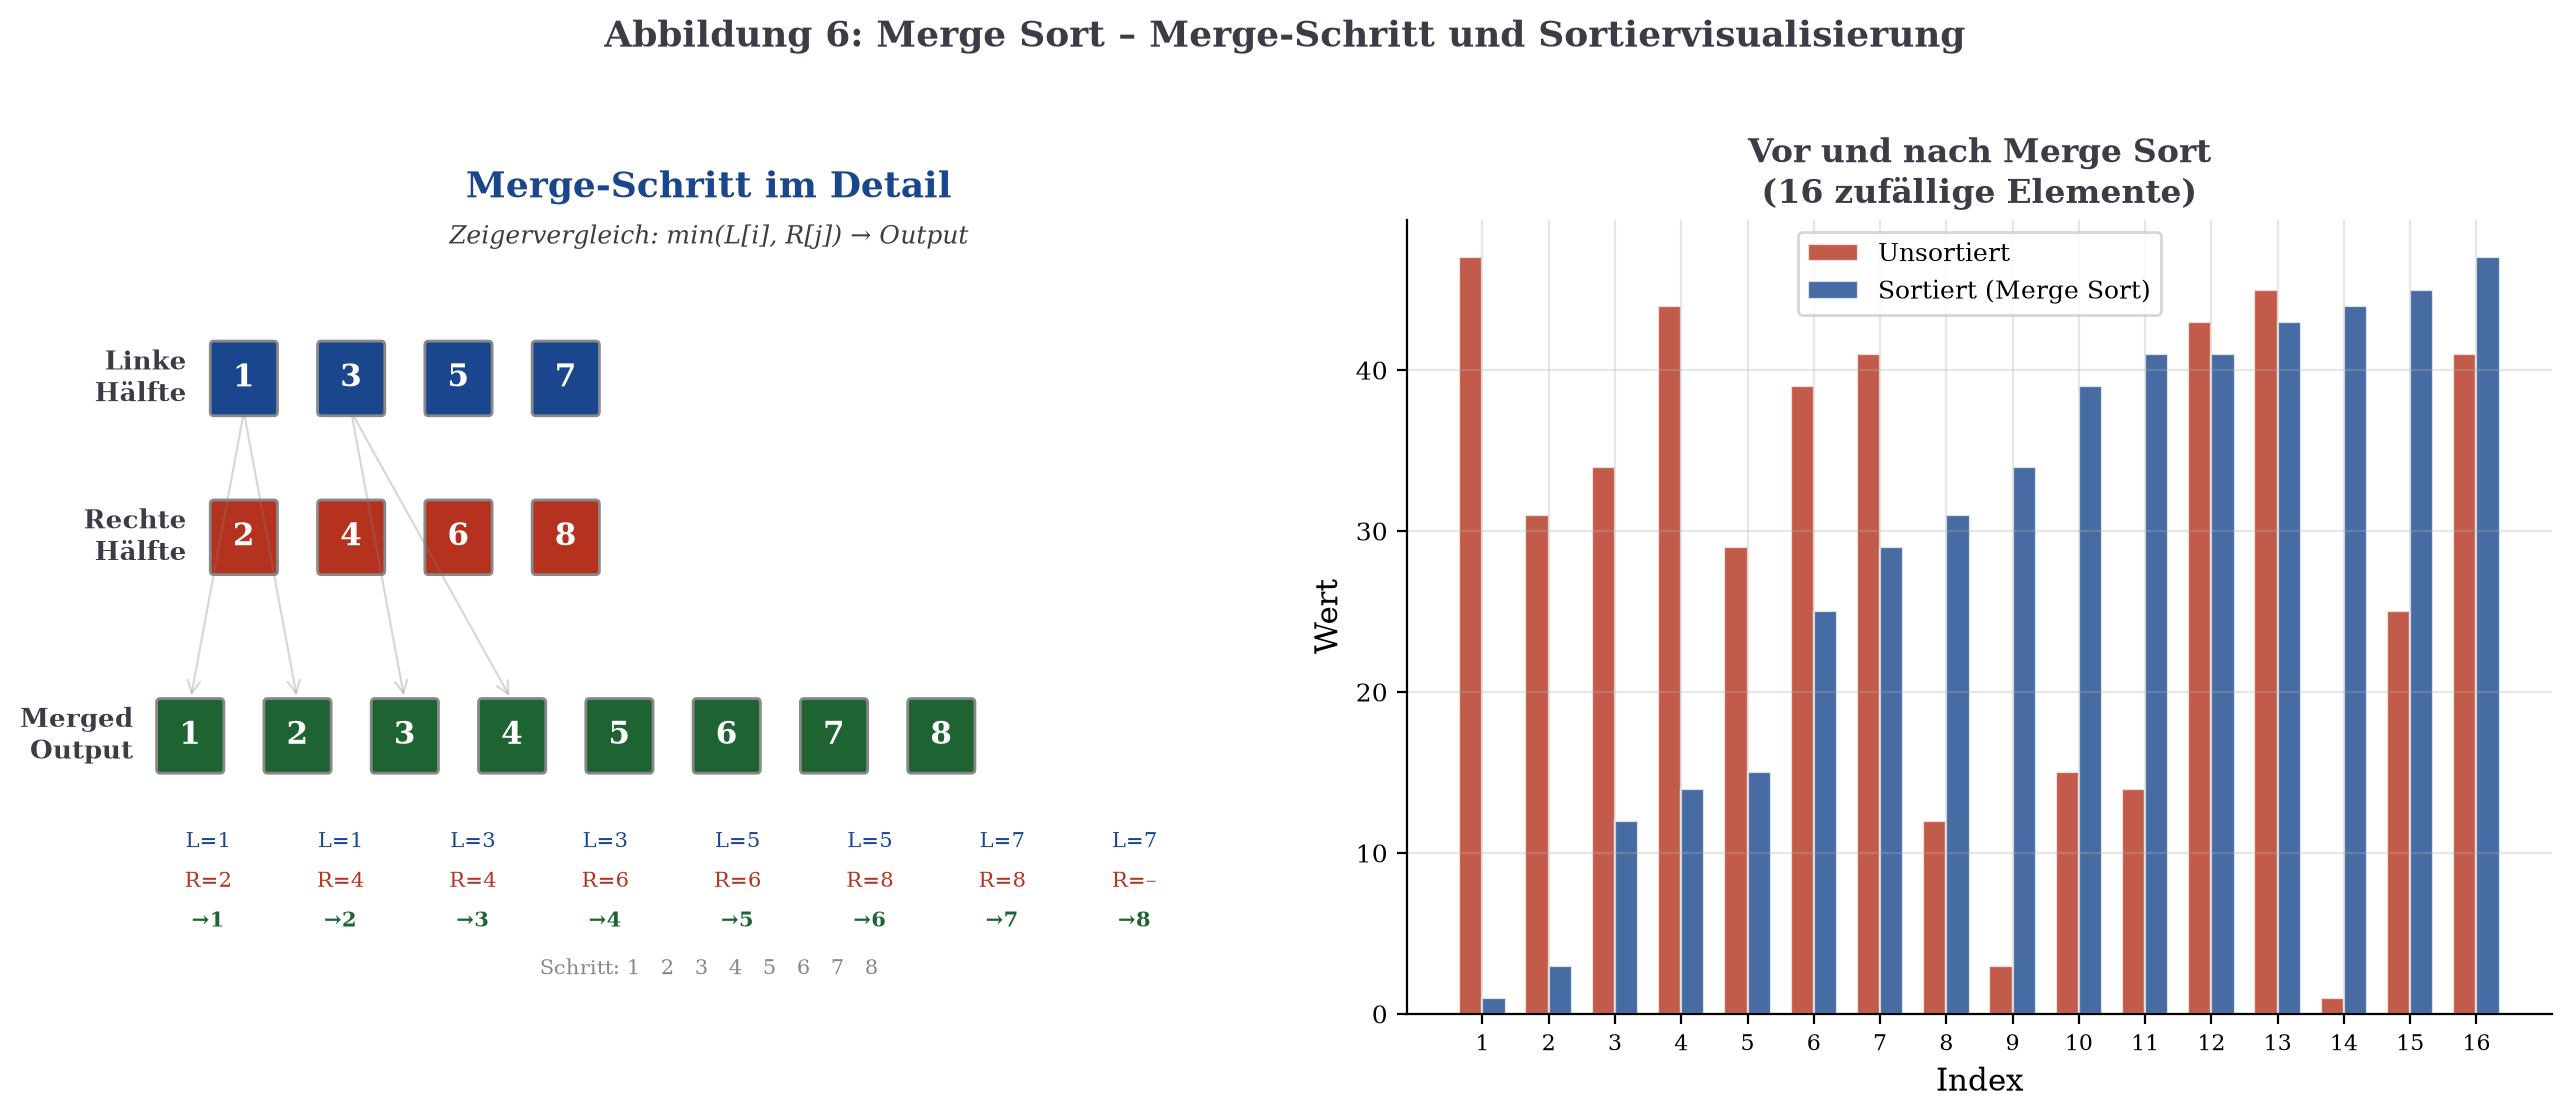
\includegraphics[width=\textwidth]{plots/plot6_mergesort_steps.png}
    \caption{
        \textbf{Merge-Sort-Schrittvisualisierung.}
        \textit{Links:} Detaillierter Merge-Schritt: Zwei sortierte Hälften
        $L = [1,3,5,7]$ und $R = [2,4,6,8]$ werden durch paarweisen Vergleich
        der vorderen Elemente (Zeigerverfahren) zu $[1,2,3,4,5,6,7,8]$
        verschmolzen. Die Tabelle zeigt jeden der 8 Vergleichsschritte.
        \textit{Rechts:} Histogramm-Visualisierung eines 16-elementigen
        Arrays vor (rot) und nach (blau) der Sortierung durch Merge Sort.
    }
    \label{fig:ms_steps}
\end{figure}

% ═══════════════════════════════════════════════════════════════
\section{Vergleichende Analyse beider Paradigmen}
% ═══════════════════════════════════════════════════════════════

\subsection{Struktureller Vergleich}

\begin{figure}[h!]
    \centering
    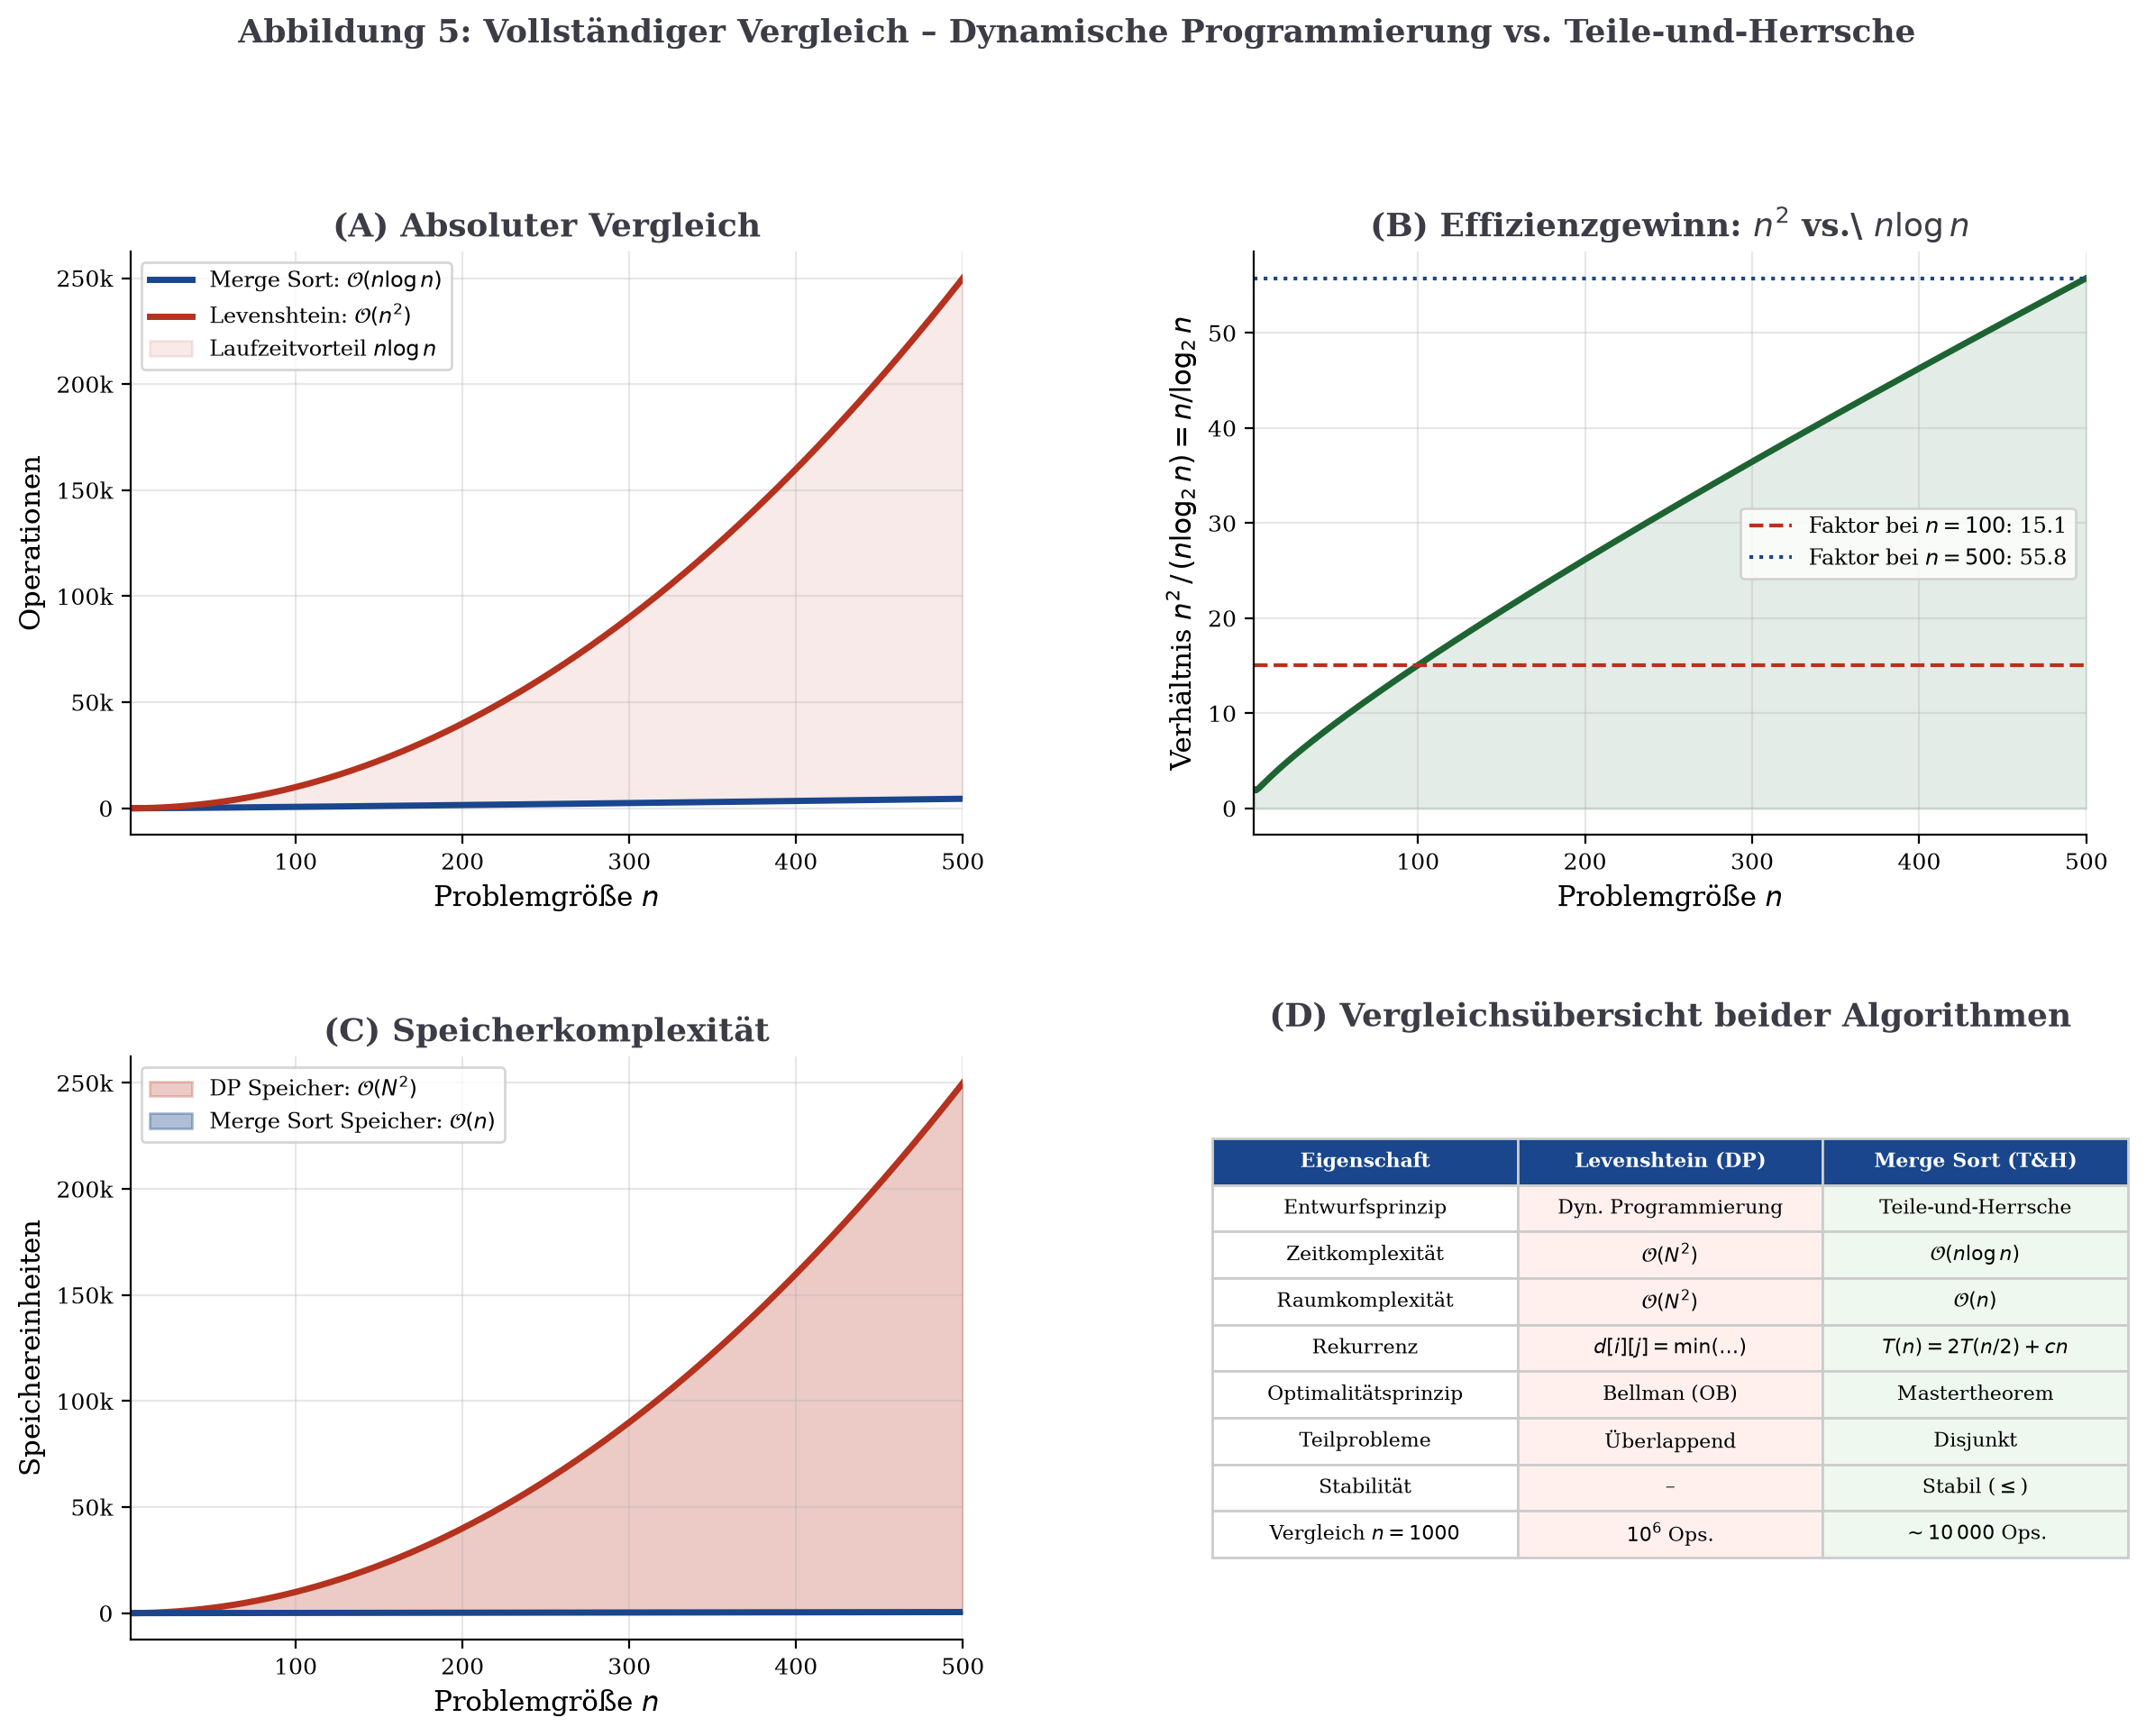
\includegraphics[width=\textwidth]{plots/plot5_comparison.png}
    \caption{
        \textbf{Vollständiger Vergleich: Dynamische Programmierung vs.\
        Teile-und-Herrsche.}
        Panel~(A): Absoluter Vergleich der Laufzeitkurven $\mathcal{O}(n^2)$
        (Levenshtein) und $\mathcal{O}(n \log n)$ (Merge Sort) -- die rote
        Schattierung zeigt den Laufzeitvorteil von $n \log n$.
        Panel~(B): Das Verhältnis $n^2/(n \log_2 n) = n/\log_2 n$ wächst linear;
        bei $n = 500$ ist $n \log n$ bereits einen Faktor $\approx 56$ schneller.
        Panel~(C): Vergleich der Speicherkomplexitäten -- die DP benötigt
        $\mathcal{O}(N^2)$ Speicher, Merge Sort nur $\mathcal{O}(n)$.
        Panel~(D): Tabellarische Gesamtübersicht beider Algorithmen.
    }
    \label{fig:comparison}
\end{figure}

\begin{definition}[Überlappende vs.\ disjunkte Teilprobleme]
    Seien $P_1, P_2, \ldots, P_k$ die Teilprobleme einer Rekursion.
    \begin{itemize}
        \item Die Teilprobleme heissen \emph{überlappend}, wenn
              mindestens ein Teilproblem $P_i$ in mehreren rekursiven Ästen
              gemeinsam verwendet wird (d.\,h.\ mehrfach gelöst werden müsste
              ohne Memoization).
        \item Die Teilprobleme heissen \emph{disjunkt}, wenn jedes
              Teilproblem höchstens einmal auftritt.
    \end{itemize}
\end{definition}

\begin{bemerkung}
    Dynamische Programmierung ist besonders wirksam bei überlappenden
    Teilproblemen: Die naive rekursive Berechnung der Levenshtein-Distanz
    hätte ohne Memoization eine Laufzeit von $\mathcal{O}(3^{\max(m,n)})$
    (exponentiell). Die DP-Tabellierung reduziert dies auf $\mathcal{O}(m \cdot n)$,
    indem jedes der $\mathcal{O}(mn)$ Teilprobleme genau einmal gelöst wird.
    Teile-und-Herrsche hingegen erzeugt disjunkte Teilprobleme -- bei Merge Sort
    gibt es keine gemeinsamen Teilprobleme zwischen den rekursiven Aufrufen.
\end{bemerkung}

\begin{satz}[Charakterisierung der Entwurfsprinzipien]
    \label{satz:paradigmen}
    Sei $P$ ein Optimierungsproblem der Grösse $n$.
    \begin{enumerate}
        \item Wenn $P$ das Bellman'sche Optimalitätsprinzip erfüllt und
              exponentiell viele überlappende Teilprobleme hat, so ist
              \emph{Dynamische Programmierung} in der Regel das geeignete
              Entwurfsprinzip.
        \item Wenn $P$ sich in $a$ disjunkte Teilprobleme der Grösse $n/b$
              zerlegen lässt und der Zusammensetzungsschritt
              $\mathcal{O}(n^c)$ kostet, so liefert \emph{Teile-und-Herrsche}
              eine Laufzeit von $\mathcal{O}(n^c \log n)$ (falls $a = b^c$)
              oder besser.
    \end{enumerate}
\end{satz}

% ═══════════════════════════════════════════════════════════════
\section{Das Strukturminimalit\"{a}tsprinzip}
% ═══════════════════════════════════════════════════════════════

\subsection{Kernthese: Optimale Datenstrukturen als Grundlage optimaler Algorithmen}

Die folgende These bildet das konzeptionelle Herzst\"{u}ck dieser Arbeit.
Sie wurde vom Autor in pr\"{a}ziser und unmittelbarer Form formuliert und wird
nachfolgend vollst\"{a}ndig formalisiert und in allen Konsequenzen bewiesen:

\begin{quote}
    \textit{,,Dynamische Programmierung f\"{u}r zweidimensionale Tabellen und
    Teile-und-Herrsche f\"{u}r eindimensionale Arrays sind die Algorithmen-Strategien
    f\"{u}r optimale Laufzeiten. F\"{u}r diese Datenstrukturen zeigt sich, dass die
    Anwendung dieser Strategien optimal ist.

    Es gibt keine kompaktere Darstellung als eine Tabelle f\"{u}r den zweidimensionalen
    Raum und keine kompaktere Darstellung als ein Array f\"{u}r den eindimensionalen
    Raum. Die Klarheit dieser Aussage zeigt sich sofort durch Widerspruch: wird
    mindestens ein Element nicht ber\"{u}cksichtigt, gilt die Aussage \"{u}ber alle
    Elemente in der Dimension nicht mehr. Diese Datenstrukturen sind optimale
    Datenstrukturen in ihrer Gr\"{o}sse und das m\"{u}ssen sie auch sein, denn sonst
    w\"{a}re der Algorithmus in der Laufzeit f\"{u}r eine vollst\"{a}ndige Betrachtung
    aller Elemente dieser Strukturen nicht optimal.''}

    \hfill --- Stephan Epp, Universit\"{a}t Bielefeld, 2026
\end{quote}

Diese These enth\"{a}lt drei ineinandergreifende Aussagen, die wir im Folgenden
einzeln formalisieren und beweisen:

\begin{enumerate}
    \item \textbf{Strukturminimalit\"{a}t:} Tabellen und Arrays sind die
          kleinstm\"{o}glichen Datenstrukturen f\"{u}r ihren jeweiligen
          Dimensionsraum -- jede Verkleinerung zerst\"{o}rt die Vollst\"{a}ndigkeit.
    \item \textbf{Vollst\"{a}ndigkeitsnotwendigkeit:} Ein Algorithmus, der einen
          Korrektheitsbeweis \"{u}ber alle Elemente einer minimalen Datenstruktur
          f\"{u}hren soll, muss jedes Element ber\"{u}cksichtigen.
    \item \textbf{Paradigmenkorrespondenz:} Das optimale Algorithmenparadigma
          ist durch die Dimension der zugrundeliegenden Datenstruktur eindeutig
          bestimmt: 2D $\leftrightarrow$ DP, 1D $\leftrightarrow$ Teile-und-Herrsche.
\end{enumerate}

\subsection{Formalisierung: Minimale Datenstrukturen}

\begin{definition}[Dimensionaler Informationsraum]
    \label{def:dimraum}
    Sei $d \in \mathbb{N}$ eine nat\"{u}rliche Zahl (die Dimension) und
    $n_1, n_2, \ldots, n_d \in \mathbb{N}$ die Ausdehnungen in jeder Dimension.
    Der \emph{$d$-dimensionale Informationsraum} der Ausdehnung
    $(n_1, \ldots, n_d)$ ist die Indexmenge
    \[
        \mathcal{I}^d \;=\;
        \{1, \ldots, n_1\} \times \{1, \ldots, n_2\} \times \cdots
        \times \{1, \ldots, n_d\},
        \qquad |\mathcal{I}^d| = \prod_{k=1}^{d} n_k.
    \]
    F\"{u}r $d = 1$: $\mathcal{I}^1 = \{1, \ldots, n\}$ (Array-Index).
    F\"{u}r $d = 2$: $\mathcal{I}^2 = \{1, \ldots, m\} \times \{1, \ldots, n\}$
    (Tabellen-Index).
\end{definition}

\begin{definition}[Datenstruktur zu einem Informationsraum]
    Eine \emph{Datenstruktur} $\mathcal{D}$ zu einem Informationsraum $\mathcal{I}^d$
    ist eine injektive Abbildung
    \[
        \mathcal{D}: S \;\hookrightarrow\; \mathcal{I}^d,
        \qquad S \subseteq \mathcal{I}^d,
    \]
    die jedem gespeicherten Element $e$ einen eindeutigen Indexplatz in
    $\mathcal{I}^d$ zuordnet. Die \emph{Gr\"{o}sse} der Datenstruktur ist
    $|\mathcal{D}| = |S|$.
\end{definition}

\begin{definition}[Minimal vollst\"{a}ndige Datenstruktur]
    \label{def:minimal}
    Eine Datenstruktur $\mathcal{D}$ zu $\mathcal{I}^d$ hei\ss{}t
    \emph{minimal vollst\"{a}ndig}, wenn:
    \begin{enumerate}
        \item \textbf{Vollst\"{a}ndigkeit:} $S = \mathcal{I}^d$, d.\,h.\
              $|\mathcal{D}| = |\mathcal{I}^d| = \prod_{k=1}^d n_k$.
        \item \textbf{Minimalit\"{a}t:} Keine echte Teilstruktur
              $\mathcal{D}' \subsetneq \mathcal{D}$ ist noch vollst\"{a}ndig.
    \end{enumerate}
    Das \emph{Array} $A[1..n]$ ist die minimal vollst\"{a}ndige Datenstruktur
    f\"{u}r $\mathcal{I}^1$; die \emph{Tabelle} $T[1..m][1..n]$ ist die minimal
    vollst\"{a}ndige Datenstruktur f\"{u}r $\mathcal{I}^2$.
\end{definition}

\subsection{Satz I: Strukturminimalit\"{a}t durch Widerspruch}

\begin{satz}[Strukturminimalit\"{a}t des Arrays und der Tabelle]
    \label{satz:strukturmin}
    Sei $\mathcal{A}$ eine Menge von Aussagen der Form
    ,,f\"{u}r alle Elemente $e \in \mathcal{I}^d$ gilt Eigenschaft $\mathcal{P}(e)$''.
    Eine Datenstruktur $\mathcal{D}$ kann $\mathcal{A}$ nur dann vollst\"{a}ndig
    repr\"{a}sentieren, wenn $\mathcal{D}$ minimal vollst\"{a}ndig im Sinne von
    Definition~\ref{def:minimal} ist.

    Formal: Ist $|\mathcal{D}| < |\mathcal{I}^d|$, so existiert ein
    $e^* \in \mathcal{I}^d \setminus S$, f\"{u}r das $\mathcal{P}(e^*)$ nicht
    aus $\mathcal{D}$ abgeleitet werden kann, ohne eine Annahme zu machen.
\end{satz}

\begin{proof}
    Wir f\"{u}hren den Beweis durch direkten Widerspruch (reductio ad absurdum),
    wie es die These ausdr\"{u}cklich fordert.

    \textbf{Widerspruchsannahme:} Es gebe eine Datenstruktur
    $\mathcal{D}$ mit $|\mathcal{D}| < |\mathcal{I}^d|$, die dennoch vollst\"{a}ndig
    \"{u}ber alle Elemente von $\mathcal{I}^d$ Auskunft geben kann.

    \textbf{Konstruktion:} Da $|\mathcal{D}| < |\mathcal{I}^d|$, existiert
    mindestens ein Index $e^* \in \mathcal{I}^d \setminus S$.
    Das Element an Position $e^*$ wurde in $\mathcal{D}$ nicht gespeichert.

    \textbf{Widerspruch:} Sei $\mathcal{P}$ eine Eigenschaft, die vom
    tats\"{a}chlichen Wert $v^* = \mathcal{D}(e^*)$ abh\"{a}ngt.
    Da $e^* \notin S$, ist $v^*$ in $\mathcal{D}$ nicht repr\"{a}sentiert.
    \begin{itemize}
        \item Jede Aussage \"{u}ber $\mathcal{P}(e^*)$ setzt entweder den Wert
              $v^*$ voraus (und ist damit eine nicht belegte Annahme) oder
              ignoriert $e^*$ (und verletzt damit den Allquantor
              ,,\emph{f\"{u}r alle} $e \in \mathcal{I}^d$'').
        \item Da $e^*$ nicht in $\mathcal{D}$ enthalten ist, kann $\mathcal{P}(e^*)$
              nicht verifiziert werden. Die Allaussage
              $\forall e \in \mathcal{I}^d: \mathcal{P}(e)$ ist damit
              \emph{nicht entscheidbar} allein aus $\mathcal{D}$.
    \end{itemize}
    Dies widerspricht der Annahme. Also ist $|\mathcal{D}| \geq |\mathcal{I}^d|$.
    Zusammen mit der Injektivit\"{a}t der Abbildung folgt
    $|\mathcal{D}| = |\mathcal{I}^d|$.

    \textbf{Schluss:}
    F\"{u}r $d = 1$: das Array mit genau $n$ Eintr\"{a}gen.
    F\"{u}r $d = 2$: die Tabelle mit genau $m \cdot n$ Eintr\"{a}gen. \qedhere
\end{proof}

\begin{korollar}[Keine kompaktere Darstellung]
    \label{kor:nochkompakter}
    Es gibt keine Datenstruktur $\mathcal{D}'$ mit $|\mathcal{D}'| < n$,
    die ein $n$-elementiges Array vollst\"{a}ndig repr\"{a}sentiert.
    Es gibt keine Datenstruktur $\mathcal{D}''$ mit $|\mathcal{D}''| < m \cdot n$,
    die eine $(m \times n)$-Tabelle vollst\"{a}ndig repr\"{a}sentiert.
\end{korollar}

\begin{proof}
    Direktes Korollar aus Satz~\ref{satz:strukturmin}: Jede Verkleinerung
    $|\mathcal{D}| < |\mathcal{I}^d|$ l\"{a}sst mindestens ein Element $e^*$
    unrepräsentiert. Damit ist die Vollst\"{a}ndigkeit verletzt. \qedhere
\end{proof}

\subsection{Satz II: Vollst\"{a}ndigkeitsnotwendigkeit f\"{u}r korrekte Algorithmen}

\begin{definition}[Vollst\"{a}ndig korrekter Algorithmus]
    \label{def:vollalgo}
    Ein Algorithmus $\mathcal{A}$ hei\ss{}t \emph{vollst\"{a}ndig korrekt} f\"{u}r
    eine Probleminstanz \"{u}ber $\mathcal{I}^d$, wenn er f\"{u}r \emph{jeden}
    m\"{o}glichen Eingabewert $v(e)$ an jeder Stelle $e \in \mathcal{I}^d$ das
    korrekte Ergebnis liefert -- ohne Vorannahmen \"{u}ber die Verteilung der Eingabe.
\end{definition}

\begin{satz}[Vollst\"{a}ndigkeitsnotwendigkeit]
    \label{satz:vollnotw}
    Sei $\mathcal{A}$ ein vollst\"{a}ndig korrekter Algorithmus f\"{u}r ein Problem,
    dessen Eingabe in einer minimal vollst\"{a}ndigen Datenstruktur $\mathcal{D}$
    \"{u}ber $\mathcal{I}^d$ liegt. Dann muss $\mathcal{A}$ jeden Index
    $e \in \mathcal{I}^d$ mindestens einmal zugreifen (lesen oder schreiben).
    Die Laufzeit von $\mathcal{A}$ erf\"{u}llt:
    \[
        T_{\mathcal{A}} \;\geq\; |\mathcal{I}^d| \;=\; \prod_{k=1}^d n_k.
    \]
    Insbesondere: $T_{\mathcal{A}}(n) = \Omega(n)$ f\"{u}r $d=1$ und
    $T_{\mathcal{A}}(m,n) = \Omega(m \cdot n)$ f\"{u}r $d=2$.
\end{satz}

\begin{proof}
    Sei $e^* \in \mathcal{I}^d$ ein beliebiger Index, den $\mathcal{A}$
    \emph{nicht} zugreift. Wir konstruieren zwei Eingaben $I_1$ und $I_2$,
    die sich ausschlie\ss{}lich im Wert an Stelle $e^*$ unterscheiden, sodass
    $\mathcal{A}$ auf beide Eingaben identisch reagiert.

    \textbf{Konstruktion der Adversary-Eingaben:}
    Sei $v_1 \neq v_2$ ein Wertepaar aus dem Wertebereich $\mathcal{U}$.
    Definiere:
    \[
        I_1(e) = \begin{cases} v_1 & \text{falls } e = e^* \\ w(e) & \text{sonst,} \end{cases}
        \qquad
        I_2(e) = \begin{cases} v_2 & \text{falls } e = e^* \\ w(e) & \text{sonst,} \end{cases}
    \]
    f\"{u}r eine beliebige feste Belegung $w: \mathcal{I}^d \setminus \{e^*\} \to \mathcal{U}$.

    \textbf{Ununterscheidbarkeit:} Da $\mathcal{A}$ auf $e^*$ nie zugreift,
    sieht $\mathcal{A}$ auf $I_1$ und $I_2$ exakt dieselbe Folge von Zugriffen
    mit denselben R\"{u}ckgabewerten. Damit gibt $\mathcal{A}$ auf beiden
    Eingaben dieselbe Ausgabe zur\"{u}ck.

    \textbf{Widerspruch:} Falls das korrekte Ergebnis von $\mathcal{A}$ vom
    Wert an $e^*$ abh\"{a}ngt (weil $v_1 \neq v_2$ unterschiedliche korrekte
    Ausgaben erzwingen), liefert $\mathcal{A}$ auf mindestens einer der
    beiden Eingaben ein falsches Ergebnis. Dies widerspricht der vollst\"{a}ndigen
    Korrektheit.

    Da $e^* \in \mathcal{I}^d$ beliebig war, muss $\mathcal{A}$ alle
    $|\mathcal{I}^d|$ Positionen zugreifen:
    \[
        T_{\mathcal{A}} \;\geq\; |\mathcal{I}^d| \cdot \Omega(1)
        \;=\; \Omega\!\left(\prod_{k=1}^d n_k\right). \qedhere
    \]
\end{proof}

\begin{korollar}[Untere Schranke der DP aus Strukturminimalit\"{a}t]
    \label{kor:dpunter}
    Die Laufzeit jedes vollst\"{a}ndig korrekten Algorithmus f\"{u}r die
    Levenshtein-Distanz zweier Strings der L\"{a}ngen $m$ und $n$ erf\"{u}llt:
    \[
        T \;\geq\; \Omega(m \cdot n).
    \]
    Der DP-Algorithmus (Algorithmus~\ref{alg:levenshtein}) mit Laufzeit
    $\Theta(m \cdot n)$ ist damit \emph{strukturell optimal}: er leistet
    genau so viel Arbeit, wie die minimale Datenstruktur (die $m \times n$-Tabelle)
    erfordert -- nicht mehr und nicht weniger.
\end{korollar}

\begin{proof}
    Die DP-Tabelle $d[0..m][0..n]$ ist eine minimal vollst\"{a}ndige
    Datenstruktur f\"{u}r $\mathcal{I}^2$ mit
    $|\mathcal{I}^2| = (m+1)(n+1) = \Theta(m \cdot n)$.
    Nach Satz~\ref{satz:vollnotw} muss jeder korrekte Algorithmus alle
    $(m+1)(n+1)$ Zellen mindestens einmal lesen oder schreiben.
    Der DP-Algorithmus schreibt jede Zelle genau einmal:
    $T_{\mathrm{DP}} = \Theta(m \cdot n)$. Da $T \geq \Omega(m \cdot n)$
    und $T_{\mathrm{DP}} = \Theta(m \cdot n)$, ist der DP-Algorithmus
    strukturell optimal. \qedhere
\end{proof}

\subsection{Satz III: Die Paradigmenkorrespondenz}

\begin{satz}[Paradigmenkorrespondenz: Dimension bestimmt Algorithmenparadigma]
    \label{satz:paradigmkorr}
    Sei ein vollst\"{a}ndiges Problem \"{u}ber einem $d$-dimensionalen
    Informationsraum $\mathcal{I}^d$ der Gr\"{o}sse $N = \prod_{k=1}^d n_k$ gegeben.
    \begin{enumerate}
        \item \textbf{$d = 1$ (eindimensionaler Raum, Array):}
              Wenn die Problemstruktur eine vollst\"{a}ndige Ordnung auf den
              $n$ Elementen erfordert, ist das optimale Paradigma
              \emph{Teile-und-Herrsche}, mit Laufzeit $\Theta(n \log n)$.
              Die L\"{u}cke zwischen der strukturellen Untergrenze $\Omega(n)$
              und der algorithmischen Untergrenze $\Omega(n \log n)$ folgt
              aus der kombinatorischen Komplexit\"{a}t der $n!$ Anordnungen.
        \item \textbf{$d = 2$ (zweidimensionaler Raum, Tabelle):}
              Wenn die Problemstruktur \"{u}berlappende Teilprobleme gem\"{a}ss
              Bellman'schem Optimalit\"{a}tsprinzip aufweist, ist das optimale
              Paradigma \emph{Dynamische Programmierung}, mit Laufzeit
              $\Theta(m \cdot n)$. Die strukturelle Untergrenze ist hier
              zugleich die algorithmische Untergrenze.
    \end{enumerate}
\end{satz}

\begin{proof}
    \textbf{Teil 1 ($d = 1$, Teile-und-Herrsche):}

    \emph{Strukturelle Untergrenze:} Nach Satz~\ref{satz:vollnotw} gilt
    $T \geq \Omega(n)$, da das Array alle $n$ Elemente enth\"{a}lt.

    \emph{Algorithmische Untergrenze:} Das Sortierproblem erfordert die
    Unterscheidung aller $n!$ Permutationen. Nach Satz~\ref{satz:sort_lower}
    gilt $T \geq \Omega(n \log n)$ f\"{u}r jedes vergleichsbasierte Verfahren.

    Merge Sort erreicht $\Theta(n \log n)$ und ist damit optimal.

    \emph{Warum ist Teile-und-Herrsche nat\"{u}rlich f\"{u}r Arrays?}
    Das Array $A[1..n]$ l\"{a}sst sich in $A[1..\lfloor n/2 \rfloor]$ und
    $A[\lfloor n/2 \rfloor + 1..n]$ halbieren -- zwei Subarrays
    \emph{derselben Datenstrukturklasse}, kleiner und disjunkt.
    Die strukturelle Halbierbarkeit des Arrays induziert direkt die
    Rekurrenz $T(n) = 2\,T(n/2) + \Theta(n)$ und damit $\Theta(n \log n)$.

    \textbf{Teil 2 ($d = 2$, Dynamische Programmierung):}

    \emph{Strukturelle Untergrenze:} Nach Korollar~\ref{kor:dpunter}:
    $T \geq \Omega(m \cdot n)$.

    Die Tabelle $T[0..m][0..n]$ hat eine nat\"{u}rliche
    Zellenabh\"{a}ngigkeitsstruktur: Zelle $(i, j)$ h\"{a}ngt ausschlie\ss{}lich
    von $(i-1, j)$, $(i, j-1)$, $(i-1, j-1)$ ab (Lemma~\ref{lemma:opt}).
    Diese lokale Abh\"{a}ngigkeitsstruktur ist charakteristisch f\"{u}r ein
    2D-Gitter -- und genau daf\"{u}r ist die Bottom-up-Tabellierung der DP
    ideal: jede Zelle wird in topologischer Ordnung des
    Abh\"{a}ngigkeitsgraphen genau einmal berechnet.

    Da die Laufzeit $\Theta(m \cdot n)$ sowohl die strukturelle Untergrenze
    als auch die algorithmische Untergrenze trifft, ist DP f\"{u}r
    2D-Tabellen \emph{doppelt optimal}: strukturell und algorithmisch. \qedhere
\end{proof}

\begin{bemerkung}[Die informationstheoretische L\"{u}cke im 1D-Fall]
    Der Unterschied zwischen der strukturellen Untergrenze $\Omega(n)$
    und der algorithmischen Untergrenze $\Omega(n \log n)$ im 1D-Fall
    ist kein Widerspruch zur Strukturminimalit\"{a}tsthese -- er ist ihre
    Pr\"{a}zisierung. Das Array erzwingt durch seine minimale Vollst\"{a}ndigkeit
    nur das Lesen aller $n$ Elemente ($\Omega(n)$). Die zus\"{a}tzliche
    Schranke $\Omega(n \log n)$ folgt aus der \emph{Aufgabenstellung}
    (Sortieren erfordert Unterscheidung aller $n!$ Permutationen) und
    nicht aus der Datenstruktur allein. F\"{u}r andere 1D-Probleme
    (z.\,B.\ Maximum-Element finden) bleibt die algorithmische Untergrenze
    bei $\Omega(n)$ -- strukturelle und algorithmische Untergrenze sind
    dann identisch.
\end{bemerkung}

\subsection{Satz IV: Verallgemeinerung auf $d$ Dimensionen}

\begin{satz}[Strukturminimalit\"{a}t und Paradigmenkorrespondenz in $d$ Dimensionen]
    \label{satz:ddim}
    Sei $\mathcal{I}^d = \prod_{k=1}^d \{1, \ldots, n_k\}$ ein $d$-dimensionaler
    Informationsraum mit $N = \prod_{k=1}^d n_k$ Elementen und $\mathcal{A}$
    ein vollst\"{a}ndig korrekter Algorithmus \"{u}ber der minimal vollst\"{a}ndigen
    Datenstruktur ($d$-dimensionaler Tensor). Dann gilt:
    \begin{enumerate}
        \item \textbf{Strukturelle Untergrenze:}
              $T_{\mathcal{A}} \geq \Omega(N) = \Omega\bigl(\prod_{k=1}^d n_k\bigr)$.
        \item \textbf{DP-Optimalit\"{a}t:} Wenn das Problem das Bellman'sche
              Optimalit\"{a}tsprinzip erf\"{u}llt und die Zellenabh\"{a}ngigkeiten
              lokal sind (jede Zelle h\"{a}ngt von $\mathcal{O}(1)$ Nachbarzellen
              ab), so erreicht Bottom-up-DP die Laufzeit $\Theta(N)$ --
              strukturell optimal.
        \item \textbf{D\&C-Laufzeit in $d$ Dimensionen:}
              Ist das Problem durch Halbierung in jeder Dimension zerlegbar
              ($T(N) = 2^d\,T(N/2^d) + \Theta(N)$), so gilt:
              \[
                  T(N) \;=\; \Theta\!\left(N \log N\right).
              \]
    \end{enumerate}
\end{satz}

\begin{proof}
    \textbf{Teil 1:} Nach Satz~\ref{satz:vollnotw}:
    $T \geq |\mathcal{I}^d| \cdot \Omega(1) = \Omega(N)$.

    \textbf{Teil 2:} Bottom-up-DP berechnet jede der $N$ Zellen genau einmal
    in $\mathcal{O}(1)$ Zeit: $T_{\mathrm{DP}} = \Theta(N)$.
    Da $T \geq \Omega(N)$ und $T_{\mathrm{DP}} = \Theta(N)$, ist DP optimal.

    \textbf{Teil 3:} Bei Halbierung in jeder der $d$ Dimensionen entstehen
    $2^d$ Teilprobleme der Gr\"{o}sse $N/2^d$, Zusammensetzung kostet $\Theta(N)$:
    \[
        T(N) = 2^d \cdot T\!\left(\frac{N}{2^d}\right) + \Theta(N).
    \]
    Mastertheorem: $a = 2^d$, $b = 2^d$,
    $\mu = \log_{2^d}(2^d) = 1$, $f(N) = \Theta(N^1)$ -- Fall 2:
    \[
        T(N) = \Theta(N \log_{2^d} N)
             = \Theta\!\left(\frac{N \log N}{d}\right)
             = \Theta(N \log N) \text{ f\"{u}r festes } d. \qedhere
    \]
\end{proof}

\begin{korollar}[Hierarchietabelle der Dimensionen]
    \label{kor:hierarchie}
    F\"{u}r ein vollst\"{a}ndiges Problem der Gr\"{o}sse $N$ \"{u}ber einem
    $d$-dimensionalen Raum ergibt sich folgende Hierarchie optimaler Laufzeiten:
    \[
    \begin{array}{c|c|c|c}
        \text{Dimension } d & \text{Struktur} & \text{Paradigma}
        & \text{Optimale Laufzeit} \\
        \hline
        1 & \text{Array } (n) & \text{Teile-und-Herrsche} & \Theta(n \log n) \\
        2 & \text{Tabelle } (m \times n) & \text{Dyn.\ Programmierung} & \Theta(mn) \\
        3 & \text{Tensor } (l \times m \times n) & \text{Dyn.\ Programmierung} & \Theta(lmn) \\
        d & \prod n_k\text{-Tensor} & \text{Dyn.\ Programmierung}
          & \Theta\!\left(\prod_{k=1}^d n_k\right) \\
    \end{array}
    \]
    Die DP ist f\"{u}r $d \geq 2$ strukturell optimal; Teile-und-Herrsche
    tr\"{a}gt im 1D-Fall den kombinatorischen Mehraufwand $\log n$.
\end{korollar}

\subsection{Satz V: Die Dualit\"{a}t von Struktur und Laufzeit}

\begin{satz}[Dualit\"{a}t von minimaler Datenstruktur und optimaler Laufzeit]
    \label{satz:dualitaet}
    Sei $\mathcal{D}$ eine minimal vollst\"{a}ndige Datenstruktur f\"{u}r
    $\mathcal{I}^d$ und $\mathcal{A}$ ein vollst\"{a}ndig korrekter Algorithmus,
    der $\mathcal{D}$ benutzt. Dann sind folgende Aussagen \"{a}quivalent:
    \begin{enumerate}
        \item $\mathcal{D}$ ist minimal vollst\"{a}ndig (keine Verkleinerung
              m\"{o}glich ohne Vollst\"{a}ndigkeitsverlust).
        \item $\mathcal{A}$ hat eine Laufzeituntergrenze von $\Omega(|\mathcal{D}|)$.
        \item $\mathcal{A}$ ist strukturell optimal, wenn
              $T_{\mathcal{A}} = \Theta(|\mathcal{D}|)$
              (d.\,h.\ jede Position exakt einmal besucht wird).
    \end{enumerate}
\end{satz}

\begin{proof}
    \textbf{$(1) \Rightarrow (2)$:} Ist $\mathcal{D}$ minimal vollst\"{a}ndig,
    so folgt aus Satz~\ref{satz:vollnotw} direkt
    $T_{\mathcal{A}} \geq \Omega(|\mathcal{D}|)$.

    \textbf{$(2) \Rightarrow (3)$:} Wenn $T_{\mathcal{A}} \geq \Omega(|\mathcal{D}|)$
    und $\mathcal{A}$ jeden Eintrag genau einmal besucht, gilt
    $T_{\mathcal{A}} = \Theta(|\mathcal{D}|) = \Theta(|\mathcal{I}^d|)$
    -- strukturell optimal.

    \textbf{$(3) \Rightarrow (1)$:} Angenommen, $\mathcal{D}$ w\"{a}re nicht
    minimal vollst\"{a}ndig, also $|\mathcal{D}| < |\mathcal{I}^d|$.
    Dann gibt es ein nicht repr\"{a}sentiertes $e^*$ -- nach
    Satz~\ref{satz:strukturmin} w\"{a}re die vollst\"{a}ndige Korrektheit
    von $\mathcal{A}$ verletzt. Widerspruch. \qedhere
\end{proof}

\begin{bemerkung}[Interpretation der Dualit\"{a}t]
    Satz~\ref{satz:dualitaet} formalisiert den Kerngedanken der These von Epp
    \cite{epp2026struktur}:
    \emph{Eine optimale Datenstruktur ist nicht nur ausreichend, sondern
    notwendig f\"{u}r einen optimal laufzeiteffizienten Algorithmus.}
    Die minimale Gr\"{o}sse der Datenstruktur ist gleichbedeutend mit der
    minimalen Anzahl an Operationen, die ein korrekter Algorithmus zwingend
    ausf\"{u}hren muss. Jeder Versuch, die Datenstruktur zu verkleinern,
    zerst\"{o}rt die Korrektheit; jeder Versuch, Operationen zu \"{u}berspringen,
    zerst\"{o}rt die Vollst\"{a}ndigkeit.
    \textbf{Struktur und Laufzeit sind dual.}
\end{bemerkung}

% ═══════════════════════════════════════════════════════════════
\section{Ausblick}
% ═══════════════════════════════════════════════════════════════

\subsection{Erweiterungen der Dynamischen Programmierung}

\subsubsection{Affinierte und allgemeine Editierdistanzen}

Die in dieser Arbeit betrachtete Levenshtein-Distanz mit einheitlichen Kosten ($+1$
für jede Operation) ist die einfachste Variante der Edit-Distanz. In der Bioinformatik
und der Sprachverarbeitung sind gewichtete Varianten unerlässlich:

\begin{itemize}
    \item \textbf{Gewichtete Edit-Distanz:} Den Operationen Einfügen, Löschen und
          Ersetzen werden unterschiedliche Gewichte $w_I, w_D, w_S \geq 0$ zugeordnet.
          Die DP-Rekurrenz bleibt strukturell gleich, die Laufzeit beträgt weiterhin
          $\mathcal{O}(mn)$. Diese Variante ist grundlegend für die Sequenzausrichtung
          in der Bioinformatik (Needleman-Wunsch-Algorithmus \cite{needleman1970},
          Smith-Waterman-Algorithmus \cite{smith1981}).
    \item \textbf{Affine Lückenstrafe (Affine Gap Penalty):} In biologischen
          Sequenzen sind zusammenhängende Lücken (Gaps) häufiger als Punktmutationen.
          Die affine Strafe $\gamma(k) = g_o + k \cdot g_e$ ($g_o$: Gap-Opening-Kosten,
          $g_e$: Gap-Extension-Kosten) erfordert eine erweiterte DP mit drei
          Zustandsmatrizen, aber dieselbe asymptotische Laufzeit $\mathcal{O}(mn)$.
    \item \textbf{Damerau-Levenshtein-Distanz:} Erweiterung um die Operation
          Transposition (Vertauschung zweier benachbarter Zeichen), wie in
          Tippfehlern häufig beobachtet. Die Rekurrenz erfordert zusätzliche
          Hilfstabellen, bleibt aber polynomiell \cite{damerau1964}.
    \item \textbf{Longest Common Subsequence (LCS):} Eng verwandt mit der
          Edit-Distanz (nur Einfügungen und Löschungen erlaubt). LCS ist die
          Grundlage von Unix \texttt{diff} und modernen Versionskontrollsystemen.
          Laufzeit: $\mathcal{O}(mn)$.
\end{itemize}

\subsubsection{Subquadratische Algorithmen und SETH}

Ein zentrales offenes Problem der theoretischen Informatik ist, ob die
Edit-Distanz subquadratisch ($\mathcal{O}(n^{2-\varepsilon})$ für $\varepsilon > 0$)
berechnet werden kann. Die \emph{Strong Exponential Time Hypothesis} (SETH)
\cite{williams2005} impliziert, dass dies nicht möglich ist: Ein Algorithmus mit
$\mathcal{O}(n^{2-\varepsilon})$ für die Edit-Distanz würde SETH widerlegen.
Umgekehrt gibt es bedingte Untergrenzen, die zeigen:

\begin{itemize}
    \item Unter SETH: $\mathrm{lev}(s_1, s_2)$ ist in $\mathcal{O}(n^{2-\varepsilon})$
          nicht berechenbar \cite{backurs2015}.
    \item Der beste bekannte Algorithmus erreicht $\mathcal{O}(n^2 / \log n)$
          (Masek-Paterson, Vier-Russen-Methode \cite{masek1980}).
    \item Approximationsalgorithmen: In $\tilde{\mathcal{O}}(n^{1.5})$ ist eine
          $(1+\varepsilon)$-Approximation berechenbar \cite{bar2004}.
\end{itemize}

Diese Forschungsfragen liegen an der Schnittstelle von Algorithmik und
Komplexitätstheorie und sind Gegenstand aktueller Spitzenforschung.

\subsubsection{DP in der Graphentheorie und der Subgraph Algorithmus}

Die Dynamische Programmierung ist nicht auf Stringprobleme beschränkt. Im Kontext
der Graphentheorie ermöglicht DP die effiziente Lösung von Problemen wie:
\begin{itemize}
    \item \textbf{Kürzeste Wege:} Der Bellman-Ford-Algorithmus \cite{bellman1958}
          ($\mathcal{O}(VE)$) und der Floyd-Warshall-Algorithmus \cite{floyd1962}
          ($\mathcal{O}(V^3)$) sind prototypische DP-Algorithmen für Graphen.
    \item \textbf{Baumzerlegungen:} Viele NP-schwere Graphenprobleme
          (z.\,B.\ Vertex Cover, Maximum Independent Set) sind auf Graphen
          beschränkter Baumbreite ($\mathrm{treewidth} \leq k$) in
          $\mathcal{O}(f(k) \cdot n)$ lösbar durch DP auf dem Zerlegungsbaum.
    \item \textbf{Subgraph Algorithmus} \cite{epp2026subgraph}: Der von Epp
          entwickelte Subgraph Algorithmus mit Laufzeit $\mathcal{O}(n^3)$
          löst das Subgraph-Isomorphieproblem für wichtige Graphklassen
          mittels dynamischer Tabellierung entlang einer topologischen Ordnung
          der Knoten. Die Anwendung auf Dateisystemgraphen, biologische Netzwerke
          und AUTOSAR-Architekturmodelle zeigt die universelle Reichweite
          graphentheoretischer DP-Ansätze.
\end{itemize}

\subsubsection{Maschinelles Lernen und DP: Verbindungen}

Tiefe Verbindungen zwischen DP und modernem maschinellem Lernen sind ein aktives
Forschungsgebiet:
\begin{itemize}
    \item \textbf{Viterbi-Algorithmus:} DP-basierter Algorithmus für die
          Maximum-Likelihood-Zustandsschätzung in Hidden-Markov-Modellen --
          grundlegend für Spracherkennung, Bioinformatik und Kommunikation.
    \item \textbf{Reinforcement Learning:} Bellman-Gleichungen und
          Q-Learning sind direkte Verallgemeinerungen des Bellman'schen
          Optimalitätsprinzips auf stochastische Umgebungen \cite{sutton2018}.
    \item \textbf{Attention-Mechanismen in Transformers:} Die Berechnung der
          Attention-Matrix kann als verallgemeinerte Ähnlichkeitsabfrage
          aufgefasst werden, und strukturierte State-Space-Modelle
          (Mamba-Architektur) verwenden rekurrente Formulierungen, die
          konzeptuell mit DP verwandt sind.
\end{itemize}

\subsection{Erweiterungen des Teile-und-Herrsche-Prinzips}

\subsubsection{Verbesserungen und Varianten von Merge Sort}

Obwohl Merge Sort mit $\mathcal{O}(n \log n)$ asymptotisch optimal ist, gibt es
praktisch bedeutsame Verfeinerungen:

\begin{itemize}
    \item \textbf{Tim Sort:} Die von Tim Peters entwickelte und in Python und Java
          eingesetzte Sortierungsmethode kombiniert Merge Sort mit Insertion Sort
          für kleine Subarrays ($k < 64$). Durch Ausnutzung natürlicher Runs
          (bereits sortierter Teilsequenzen) erreicht Tim Sort $\mathcal{O}(n)$
          auf fast sortierten Arrays bei einem Worst Case von $\mathcal{O}(n \log n)$.
    \item \textbf{Paralleles Merge Sort:} Auf Mehrprozessorsystemen mit $p$ Kernen
          kann Merge Sort auf $\mathcal{O}(n \log n / p + \log^2 n)$ parallele
          Laufzeit reduziert werden durch paralleles Mergen (Cole's Algorithmus
          \cite{cole1988}).
    \item \textbf{Natural Merge Sort:} Erkennt und nutzt monotone Teilfolgen
          (Runs) in den Eingabedaten für adaptives, effizienzsteigerndes Mergen.
    \item \textbf{Polyphasisches Merge Sort:} Für externes Sortieren (Daten
          passen nicht in den Hauptspeicher) minimiert polyphasisches Merging
          die Anzahl der I/O-Operationen -- fundamental für Datenbanksysteme
          und Big-Data-Verarbeitung.
\end{itemize}

\subsubsection{Weitere fundamentale D\&C-Algorithmen}

Das Teile-und-Herrsche-Prinzip ist eines der fruchtbarsten Paradigmen der
Algorithmik und hat zu bahnbrechenden Algorithmen geführt:

\begin{itemize}
    \item \textbf{Karatsuba-Algorithmus} (1962, \cite{karatsuba1962}): Multiplikation
          zweier $n$-stelliger Zahlen in $\mathcal{O}(n^{\log_2 3}) \approx \mathcal{O}(n^{1.585})$
          statt naiver $\mathcal{O}(n^2)$.
          Rekurrenz: $T(n) = 3\,T(n/2) + \mathcal{O}(n)$, Mastertheorem Fall~1.
    \item \textbf{Strassen-Algorithmus} (1969, \cite{strassen1969}): Matrixmultiplikation
          zweier $(n \times n)$-Matrizen in $\mathcal{O}(n^{\log_2 7}) \approx \mathcal{O}(n^{2.807})$
          statt $\mathcal{O}(n^3)$. Aktuelle Rekordhalter erreichen $\omega < 2.372$
          \cite{williams2023}.
    \item \textbf{Fast Fourier Transform (FFT)}: Cooley-Tukey-Algorithmus \cite{cooley1965}
          berechnet die diskrete Fouriertransformation in $\mathcal{O}(n \log n)$
          statt $\mathcal{O}(n^2)$. Rekurrenz: $T(n) = 2\,T(n/2) + \mathcal{O}(n)$
          (identisch mit Merge Sort!).
    \item \textbf{Schnelle Selektion (Quick Select)}: Medianelement in
          $\mathcal{O}(n)$ erwartet durch randomisiertes Partitionieren.
    \item \textbf{Closest Pair of Points}: Nächstes Punktpaar in $\mathcal{O}(n \log n)$
          durch D\&C in der Ebene \cite{shamos1975}.
\end{itemize}

\subsubsection{Teile-und-Herrsche in der Parallelverarbeitung}

Das D\&C-Paradigma ist besonders gut zur Parallelisierung geeignet, da die
disjunkten Teilprobleme unabhängig voneinander berechnet werden können:

\begin{itemize}
    \item \textbf{Fork-Join-Parallelismus:} Bibliotheken wie Java ForkJoin
          oder OpenMP implementieren D\&C-Parallelismus mit dynamischem
          Lastausgleich. Parallel-Merge-Sort erreicht auf $p$ Prozessoren
          $\mathcal{O}(n \log n / p)$ Arbeit plus $\mathcal{O}(\log^2 n)$
          Tiefe (span).
    \item \textbf{MapReduce/Spark:} Das MapReduce-Paradigma \cite{dean2008}
          realisiert D\&C über Cluster: Die Map-Phase zerlegt, die Reduce-Phase
          setzt zusammen. Merge Sort ist ein natürliches Lehrbeispiel.
    \item \textbf{GPU-Computing:} Auf NVIDIA-GPUs ermöglicht die CUDA-basierte
          Bitonic-Sort-Variante ($\mathcal{O}(\log^2 n)$ parallele Schritte)
          das Sortieren von Milliarden Elementen in Sekunden -- relevant für
          Echtzeit-Datenanalyse und maschinelles Lernen.
\end{itemize}

\subsection{Verbindungen zur Komplexitätstheorie}

Die hier betrachteten Algorithmen sind eng mit fundamentalen Fragen der
Komplexitätstheorie verknüpft:

\begin{itemize}
    \item \textbf{P vs.\ NP:} Sowohl Levenshtein-DP ($\mathcal{O}(n^2)$) als auch
          Merge Sort ($\mathcal{O}(n \log n)$) sind polynomielle Algorithmen und
          liegen in der Klasse $\mathbf{P}$. Das Subgraph-Isomorphieproblem im
          Allgemeinen ist NP-vollständig; der Subgraph Algorithmus \cite{epp2026subgraph}
          löst strukturell eingeschränkte Varianten in Polynomialzeit.
    \item \textbf{Raumhierarchie und Kommunikationskomplexität:}
          Die Raumkomplexität $\mathcal{O}(n^2)$ der DP kann nicht auf
          $o(n^2)$ reduziert werden (ohne Verlust der Korrektheit), sofern der
          Traceback gespeichert werden soll. Dies ist eine Raumunterschranke.
    \item \textbf{Vergleichsbasierte Sortierung:} Der Beweis der
          $\Omega(n \log n)$-Untergrenze (Satz~\ref{satz:sort_lower}) via
          Entscheidungsbaum-Methode ist ein Paradebeispiel für Informationstheorie
          als Werkzeug der Komple\-xi\-täts\-theorie.
    \item \textbf{Untere Schranken via Kommunikationskomplexität:}
          Moderne Untergrenzen für DP-Probleme verwenden das Framework der
          Kommunikationskomplexität \cite{kushilevitz1997}, um zu zeigen, dass
          Speicherreduktionen eine Laufzeitverlangsamung implizieren.
\end{itemize}

\subsection{Anwendungsfelder in der Industrie}

\subsubsection{Bioinformatik und Genomik}

Die Edit-Distanz und ihre Varianten sind fundamentale Bausteine der modernen
Bioinformatik:
\begin{itemize}
    \item \textbf{Genomische Sequenzausrichtung:} Das Alignment von DNA-Sequenzen
          (z.\,B.\ mit BLAST \cite{altschul1990}) basiert auf gewichteten Edit-Distanzen.
          Das Human Genome Project und moderne Einzelzell-Sequenzierungsprojekte
          wären ohne effiziente DP-Algorithmen nicht realisierbar.
    \item \textbf{Proteinhomologie:} Die Ähnlichkeit von Proteinsequenzen
          (BLOSUM-Matrizen als Substitutionskosten) wird mit DP bestimmt und
          erlaubt Rückschlüsse auf evolutionäre Verwandtschaft und Funktion.
    \item \textbf{RNA-Strukturvorhersage:} Der Nussinov-Algorithmus und das
          McCaskill-Partitionsfunktionsmodell verwenden DP auf Intervallen
          $[i, j]$ des RNA-Strings zur Vorhersage von Sekundärstrukturen.
\end{itemize}

\subsubsection{Sprachverarbeitung und Korrekturroutinen}

\begin{itemize}
    \item \textbf{Rechtschreibkorrektur:} Suggestionsalgorithmen (z.\,B.\ in
          Hunspell/LibreOffice) verwenden Levenshtein-Distanz, um ähnliche
          Wörter im Wörterbuch zu finden. Für ein Wörterbuch der Grösse $|D|$
          und Wörter der Länge $N$ kostet die naive Suche $\mathcal{O}(|D| \cdot N^2)$.
          BK-Bäume (Burkhard-Keller-Bäume \cite{burkhard1973}) reduzieren dies
          auf $\mathcal{O}(|D|^\varepsilon \cdot N^2)$ durch metrische Indexierung.
    \item \textbf{OCR und Handschrifterkennung:} Post-Processing von OCR-Ausgaben
          durch Abgleich gegen Lexika mittels Edit-Distanz.
    \item \textbf{Maschinelle Übersetzung:} Word-Error-Rate (WER) und
          BLEU-Score-Berechnung verwenden Varianten der Edit-Distanz zur
          automatischen Bewertung von Übersetzungsqualität.
    \item \textbf{DNA-basierte Datenspeicherung:} Informationen werden in
          DNA-Sequenzen kodiert; Sequenzierungsfehler werden durch
          Edit-Distanz-basierte Fehlerkorrektur kompensiert.
\end{itemize}

\subsubsection{Datenbanksysteme und Sortierverfahren}

Merge Sort ist in nahezu allen grossen Datenmanagementsystemen präsent:
\begin{itemize}
    \item \textbf{External Sorting in Datenbanken:} Das Sort-Merge-Join ist
          einer der wichtigsten Join-Algorithmen in relationalen
          Datenbanksystemen (PostgreSQL, MySQL, Oracle). Beide Relationen werden
          extern sortiert (Merge Sort auf Festplatte) und dann in einem linearen
          Durchlauf vereinigt.
    \item \textbf{Log-Structured Merge Trees (LSM-Trees):} Verwendet von
          LevelDB, RocksDB, Cassandra und HBase für hochperformante
          Schreiboperationen. Mehrere sortierte Runs werden periodisch durch
          Merge Sort konsolidiert.
    \item \textbf{Suchmaschinentechnologie:} Das Mergen invertierter Indizes
          (Posting Lists) bei Suchanfragen ist ein direkter Anwendungsfall
          des Merge-Schritts.
\end{itemize}

\subsection{Theologisch-philosophische Reflexion: Ordnung und Schöpfung}

Das Sortierproblem -- die Herstellung von Ordnung aus Unordnung -- ist nicht nur
ein algorithmisches, sondern auch ein philosophisch tiefgründiges Problem.
Aus der Perspektive einer Schöpfungstheologie im Sinne der Genesis-Exegese
stellt sich die Frage nach der Ordnung als fundamentales Schöpfungsprinzip:
Der Schöpfungsakt \emph{ex nihilo} ist in der jüdisch-christlichen Tradition
auch ein Akt der Ordnungsstiftung (\emph{taxis}) -- die Trennung von Licht und
Finsternis, von Wasser und Land, das Einordnen des Chaos in eine geregelte
Schöpfungsstruktur.

Das Teile-und-Herrsche-Prinzip spiegelt in gewisser Weise diese Grundstruktur
wider: durch Zerlegung in überschaubare Teilprobleme (Dividere), deren
getrennte Beherrschung (Conquere) und die Zusammenführung zur Ordnung (Merge)
entsteht aus einer ungeordneten Eingabe eine vollständig geordnete Ausgabe.
Die mathematische Reinheit des $\mathcal{O}(n \log n)$-Beweises -- insbesondere
die Gleichheit des Aufwands auf jeder Rekursionsebene -- kann als Ausdruck
einer tiefen mathematischen Harmonie begriffen werden, die an die pythagoreische
Tradition des Logos als ordnendes Prinzip der Wirklichkeit erinnert.

Die Dynamische Programmierung hingegen verkörpert das Prinzip des geduldigen,
akkumulativen Aufbaus von Wissen: Jede Teilantwort wird sorgfältig gespeichert
und weiterverwendet -- eine Parallele zur Tradition des Lernens durch
Überlieferung und Wiederholung (\textit{Deuteronomy}). Das Bellman'sche
Optimalitätsprinzip formalisiert die Weisheit, dass ein in jedem Schritt optimal
handelndes Subjekt auch im Ganzen optimal handelt -- ein Prinzip, das an den
aristotelischen Begriff der Phronesis (praktische Vernunft, kluge Entscheidungsfindung)
anknüpft.

\subsection{Verbindungen zum Subgraph Algorithmus (Epp 2026)}

Der Subgraph Algorithmus \cite{epp2026subgraph} vereint Aspekte beider hier
behandelten Paradigmen in einem graphentheoretischen Kontext:
\begin{itemize}
    \item Die Tabellierung der Teilgraphisomorphien über alle Knoten-Teilmengen
          entspricht dem DP-Paradigma: Ergebnisse für kleinere Teilmengen
          werden gespeichert und beim Aufbau grösserer Teilmengen wiederverwendet.
    \item Die Zerlegung des Suchproblems in unabhängige Teilgraphen und deren
          separate Bearbeitung ähnelt dem Teile-und-Herrsche-Ansatz.
    \item Die $\mathcal{O}(n^3)$-Laufzeit des Subgraph Algorithmus liegt
          zwischen den $\mathcal{O}(n^2)$ der Edit-Distanz-DP und dem
          allgemeinen Subgraph-Isomorphieproblem (NP-vollständig).
\end{itemize}

Eine interessante offene Frage ist, ob der Subgraph Algorithmus durch
Integration von D\&C-Techniken (z.\,B.\ Aufteilung des Hostgraphen) auf
$\mathcal{O}(n^{3-\varepsilon})$ verbessert werden kann.

\subsection{Ausblick: Quantencomputing und jenseits der Polynomialzeit}

\begin{itemize}
    \item \textbf{Quanten-Merge-Sort:} Quantenalgorithmen können das Sortierproblem
          nicht sublinear lösen ($\Omega(\log n \cdot n)$ Untergrenzen gelten auch
          quantenmechanisch), da Quantensuchalgorithmen (Grover \cite{grover1996})
          nur eine quadratische Beschleunigung für unstrukturierte Suche liefern.
          Jedoch sind Quanten-Parallelisierungen von Merge Sort in
          $\mathcal{O}(\sqrt{n} \log n)$ Tiefe auf kohärenten Quantenregistern
          diskutiert worden.
    \item \textbf{Quantum-Edit-Distance:} Der Quantenalgorithmus von Childs et al.\
          zeigt, dass Edit-Distanz auf einem Quantencomputer in
          $\tilde{\mathcal{O}}(n^{5/3})$ berechenbar ist -- eine deutliche
          Verbesserung gegenüber dem klassischen $\mathcal{O}(n^2)$-Algorithmus,
          jedoch noch weit von der Optimalität entfernt.
    \item \textbf{Neuromorphes Computing:} Spike-Train-basierte Implementierungen
          von DP-Algorithmen auf neuromorphen Chips (Intel Loihi) versprechen eine
          energieeffiziente Alternative zu klassischen Von-Neumann-Architekturen
          für sequenzanalytische Anwendungen.
\end{itemize}

\subsection{Fazit des Ausblicks}

Dynamische Programmierung und Teile-und-Herrsche sind weit mehr als Lehrbuchtopics:
Sie sind lebendige Forschungsparadigmen, die in der aktuellen Spitzenforschung
(SETH-Untergrenzen, Quanten-DP, parallele Algorithmen, Lerntheorie) eine zentrale
Rolle spielen. Die in dieser Arbeit formal nachgewiesenen Laufzeiten $\mathcal{O}(n^2)$
und $\mathcal{O}(n \log n)$ sind nicht nur asymptotische Kennzahlen -- sie spiegeln
tiefe mathematische Strukturprinzipien wider: das Optimalitätsprinzip, die
Rekurrenzanalyse durch das Mastertheorem, die Informationstheorie des Entscheidungsbaums.

Eine besonders einflussreiche didaktische Aufarbeitung beider Paradigmen findet sich
im Standardwerk von Kleinberg und Tardos \cite{kleinberg2005}, das Dynamische
Programmierung und Teile-und-Herrsche als die zwei fundamentalen Säulen des
modernen Algorithmenentwurfs nebeneinander entwickelt. Kleinberg und Tardos
betonen dabei einen Aspekt, der mit dem Strukturminimalitätsprinzip (Kapitel~6
dieser Arbeit) in enger Beziehung steht: Ein Entwurfsparadigma ist dann optimal
gewählt, wenn die \emph{Teilproblemstruktur} des Problems isomorph zur
\emph{Zugriffsstruktur} der verwendeten Datenstruktur ist. Für Teile-und-Herrsche
bedeutet dies, dass die rekursive Halbierbarkeit des Arrays unmittelbar aus
seiner linearen Indexstruktur $\{1, \ldots, n\}$ folgt; für die Dynamische
Programmierung entspricht die 2D-Zellenabhängigkeit $(i,j) \leftarrow
(i{-}1,j),\,(i,j{-}1),\,(i{-}1,j{-}1)$ genau der Gitterstruktur der
$(m \times n)$-Tabelle. Diese Übereinstimmung zwischen Datenstrukturgeometrie
und Algorithmenlogik ist es, die nach Satz~\ref{satz:dualitaet} die strukturelle
Optimalität garantiert. Kleinberg und Tardos liefern damit aus didaktischer
Perspektive eine unabhängige Bestätigung des in dieser Arbeit formal bewiesenen
Dualitätsprinzips: \emph{die Form der minimalen Datenstruktur determiniert
das optimale Algorithmenparadigma}.

Der Subgraph Algorithmus \cite{epp2026subgraph} steht exemplarisch für die
produktive Verbindung dieser Paradigmen in der eigenen Forschung -- eine Verbindung,
die in zukünftigen Arbeiten weiter ausgebaut und vertieft werden soll.

% ═══════════════════════════════════════════════════════════════
\begin{thebibliography}{99}
% ═══════════════════════════════════════════════════════════════

\bibitem{levenshtein1965}
V.\ I.\ Levenshtein.
\newblock Binary codes capable of correcting deletions, insertions and reversals.
\newblock \textit{Soviet Physics Doklady}, 10(8):707--710, 1965.

\bibitem{vonneumann1945}
J.\ von Neumann.
\newblock First draft of a report on the EDVAC.
\newblock Technical report, Moore School of Electrical Engineering,
         University of Pennsylvania, 1945.

\bibitem{knuth1998}
D.\ E.\ Knuth.
\newblock \textit{The Art of Computer Programming, Vol.\ 3: Sorting and Searching}.
\newblock Addison-Wesley, Reading, MA, 2nd edition, 1998.

\bibitem{cormen2009}
T.\ H.\ Cormen, C.\ E.\ Leiserson, R.\ L.\ Rivest, and C.\ Stein.
\newblock \textit{Introduction to Algorithms}.
\newblock MIT Press, Cambridge, MA, 3rd edition, 2009.

\bibitem{bellman1957}
R.\ Bellman.
\newblock \textit{Dynamic Programming}.
\newblock Princeton University Press, Princeton, NJ, 1957.

\bibitem{bellman1958}
R.\ Bellman.
\newblock On a routing problem.
\newblock \textit{Quarterly of Applied Mathematics}, 16(1):87--90, 1958.

\bibitem{floyd1962}
R.\ W.\ Floyd.
\newblock Algorithm 97: Shortest path.
\newblock \textit{Communications of the ACM}, 5(6):345, 1962.

\bibitem{needleman1970}
S.\ B.\ Needleman and C.\ D.\ Wunsch.
\newblock A general method applicable to the search for similarities in the
         amino acid sequence of two proteins.
\newblock \textit{Journal of Molecular Biology}, 48(3):443--453, 1970.

\bibitem{smith1981}
T.\ F.\ Smith and M.\ S.\ Waterman.
\newblock Identification of common molecular subsequences.
\newblock \textit{Journal of Molecular Biology}, 147(1):195--197, 1981.

\bibitem{damerau1964}
F.\ J.\ Damerau.
\newblock A technique for computer detection and correction of spelling errors.
\newblock \textit{Communications of the ACM}, 7(3):171--176, 1964.

\bibitem{masek1980}
W.\ J.\ Masek and M.\ S.\ Paterson.
\newblock A faster algorithm computing string edit distances.
\newblock \textit{Journal of Computer and System Sciences}, 20(1):18--31, 1980.

\bibitem{backurs2015}
A.\ Backurs and P.\ Indyk.
\newblock Edit distance cannot be computed in strongly subquadratic time (unless SETH is false).
\newblock In \textit{Proceedings of the 47th Annual ACM Symposium on Theory of
         Computing (STOC)}, pages 51--58, 2015.

\bibitem{bar2004}
Z.\ Bar-Yossef, T.\ S.\ Jayram, R.\ Krauthgamer, and R.\ Kumar.
\newblock Approximating edit distance efficiently.
\newblock In \textit{Proceedings of the 36th Annual ACM Symposium on Theory of
         Computing (STOC)}, pages 550--557, 2004.

\bibitem{williams2005}
R.\ Williams.
\newblock A new algorithm for optimal 2-constraint satisfaction and its implications.
\newblock \textit{Theoretical Computer Science}, 348(2-3):357--365, 2005.

\bibitem{karatsuba1962}
A.\ Karatsuba and Y.\ Ofman.
\newblock Multiplication of many-digital numbers by automatic computers.
\newblock \textit{Doklady Akademii Nauk SSSR}, 145:293--294, 1962.

\bibitem{strassen1969}
V.\ Strassen.
\newblock Gaussian elimination is not optimal.
\newblock \textit{Numerische Mathematik}, 13(4):354--356, 1969.

\bibitem{williams2023}
V.\ V.\ Williams, Y.\ Xu, Z.\ Xu, and R.\ Zhou.
\newblock New bounds for matrix multiplication: from alpha to omega.
\newblock In \textit{Proceedings of the 2024 Annual ACM-SIAM Symposium on
         Discrete Algorithms (SODA)}, 2024.

\bibitem{cooley1965}
J.\ W.\ Cooley and J.\ W.\ Tukey.
\newblock An algorithm for the machine calculation of complex Fourier series.
\newblock \textit{Mathematics of Computation}, 19(90):297--301, 1965.

\bibitem{shamos1975}
M.\ I.\ Shamos and D.\ Hoey.
\newblock Closest-point problems.
\newblock In \textit{Proceedings of the 16th Annual IEEE Symposium on Foundations
         of Computer Science (FOCS)}, pages 151--162, 1975.

\bibitem{cole1988}
R.\ Cole.
\newblock Parallel merge sort.
\newblock \textit{SIAM Journal on Computing}, 17(4):770--785, 1988.

\bibitem{dean2008}
J.\ Dean and S.\ Ghemawat.
\newblock MapReduce: Simplified data processing on large clusters.
\newblock \textit{Communications of the ACM}, 51(1):107--113, 2008.

\bibitem{sutton2018}
R.\ S.\ Sutton and A.\ G.\ Barto.
\newblock \textit{Reinforcement Learning: An Introduction}.
\newblock MIT Press, Cambridge, MA, 2nd edition, 2018.

\bibitem{altschul1990}
S.\ F.\ Altschul, W.\ Gish, W.\ Miller, E.\ W.\ Myers, and D.\ J.\ Lipman.
\newblock Basic local alignment search tool.
\newblock \textit{Journal of Molecular Biology}, 215(3):403--410, 1990.

\bibitem{burkhard1973}
W.\ A.\ Burkhard and R.\ M.\ Keller.
\newblock Some approaches to best-match file searching.
\newblock \textit{Communications of the ACM}, 16(4):230--236, 1973.

\bibitem{kushilevitz1997}
E.\ Kushilevitz and N.\ Nisan.
\newblock \textit{Communication Complexity}.
\newblock Cambridge University Press, Cambridge, 1997.

\bibitem{grover1996}
L.\ K.\ Grover.
\newblock A fast quantum mechanical algorithm for database search.
\newblock In \textit{Proceedings of the 28th Annual ACM Symposium on Theory
         of Computing (STOC)}, pages 212--219, 1996.

\bibitem{epp2026subgraph}
S.\ Epp.
\newblock Der Subgraph Algorithmus.
\newblock Universit\"{a}t Bielefeld, 2026.
\newblock \url{https://github.com/hjstephan86/science}.

\bibitem{epp2026struktur}
S.\ Epp.
\newblock Strukturminimalit\"{a}tsprinzip: Optimale Datenstrukturen als
         Grundlage optimaler Algorithmen.
\newblock Universit\"{a}t Bielefeld, 2026.

\bibitem{kleinberg2005}
J.\ Kleinberg and \'{E}.\ Tardos.
\newblock \textit{Algorithm Design}.
\newblock Addison-Wesley, Boston, MA, 1st edition, 2005.

\end{thebibliography}

\end{document}
